\begin{landscape}

\chapter{Testing}

\section{Test Plan}

\subsection{Original Outline Plan}

\begin{center}
    \begin{tabular}{|p{2cm}|p{5cm}|p{5cm}|p{4cm}|}
        \hline
        \textbf{Test Series} & \textbf{Purpose of Test Series} & \textbf{Testing Strategy} & \textbf{Strategy Rationale}\\ \hline
        1 & Testing the flow of control between user interfaces & Top-down Testing & \\ \hline
        2 & Testing the validation of input data & Bottom-up testing & All components are to be tested after development \\ \hline
        3 & Testing the algorithms' functionality & White box testing & \\ \hline
        4 & Testing that the information has been successfully stored, and in the right places & Black box testing & \\ \hline
        5 & Testing the system and whether it meets the requirements & System testing & \\ \hline
    \end{tabular}
\end{center}


\subsection{Changes to Outline Plan}

There were no changes the the purposes of the the test series and strategies, however I have added all the strategy rationales.

\begin{center}
    \begin{tabular}{|p{2cm}|p{5cm}|p{5cm}|p{4cm}|}
        \hline
        \textbf{Test Series} & \textbf{Purpose of Test Series} & \textbf{Testing Strategy} & \textbf{Strategy Rationale}\\ \hline 
        1 & Testing the flow of control between user interfaces & Top-down Testing & Tests the outputs alone, disregarding internal functionality \\ \hline
        2 & Testing the validation of input data & Bottom-up testing & Components will be tested after development \\ \hline
        3 & Testing the algorithms' functionality & White box testing & Components will be tested after development \\ \hline
        4 & Testing that the information has been successfully stored, and in the right places & Black box testing & Focuses on the process of adding/editing/deleting data \\ \hline
        5 & Testing the system and whether it meets the requirements & System testing & Tests the flow of control with all components breifly tested \\ \hline
    \end{tabular}
\end{center}

\subsection{Original Detailed Plan}


\begin{center}
    \begin{longtable}{|p{1.5cm}|p{2cm}|p{2.5cm}|p{2.5cm}|p{2cm}|p{2cm}|p{2cm}|p{2cm}|}
        \hline
        \textbf{Test Series} & \textbf{Purpose of Test} & \textbf{Test Description} & \textbf{Test Data} & \textbf{Test Data Type (Normal/ Erroneous/ Boundary)} & \textbf{Expected Result} & \textbf{Actual Result} & \textbf{Evidence}\\ \hline
        1.1 & Test the Log in button on the log in screen & This should check whether the password and email match and exist in a record & Click the log in button & Normal & If the email and password match, the main menu should open, else the program should prompt the user with an error & & \\ \hline
        1.2 & Test the View button on the main menu & This button links the main menu to the view menu. & Click the View Button & Normal & The program should open the View Menu in a new window & & \\ \hline
        1.3 & Testing the Log Out button on the Main Menu & This button links to the Login screen, where the user is required to log in again & Click the Log out button & Normal & The screen should switch to the log out screen & & \\ \hline
        1.4 & Testing the Search Database button on the Main Menu & This button should prompt a seperate interface to open, and show details which can be used to search for specific items in the database & Click the Search Database button & Normal & The program should open a new window consisting of the Search Database screen & & \\ \hline
        1.5 & Testing the Add Entry button on the Main Menu & This button should prompt a seperate interface to open and show the Add Entry screen & Click the Add Entry button & Normal & The program should open the Add Entry screen in a new window & & \\ \hline
        1.6 & Testing the Edit Entry button from the Main Menu & This button links to the Editing screen & Click the Edit Entry button & Normal & The program should switch to the Editing screen from the Main Menu &  & \\ \hline
        1.7 & Testing the Edit Entry button after an entry has been selected beforehand & These conditions should open the Edit Entry screen upon clicking Edit Entry, with data on the selected entry already filled in on the grid & Click on an entry, and then click Edit Entry & Normal & The program should open the Edit Entry screen in a new window & & \\ \hline
        1.8 & Testing the Remove Entry Button after an entry has been selected beforehand & These conditions should prompt the user for verification on deleting a selected customer record & Click on an entry and then click Remove Entry & Normal & The program should open a Verification window, asking the user for confirmation and verification on removing the selected customer record & & \\ \hline
        1.9 & Testing the Change Password Button on the Main Menu & This button prompts the Change Password window to open & Click the Change Password button & Normal & The program should open the Change Password window, with fields required to be filled in in order to change the password & & \\ \hline
        1.10 & Testing the Quick Search button on the Main Menu & This button returns the customer that matches the entered AuthorID & Type in a Lastname and click QuickSearch & Normal & The program should return the customer that matches the entered Lastname and show it in the grid & & \\ \hline
        1.11 & Testing the back button on the View Menu & This button returns back to the main menu & Click Back & Normal & The program should return back to the main menu & & \\ \hline
        1.12 & Testing the Add Book Button on the View Menu & This button opens up a new window for adding a book & Click Add Book & Normal & The program should open a new window for adding a book & & \\ \hline
        1.13 & Testing the View Publishing Invoice button on the View Menu & This button opens up a new window displaying details about the selected book's publishing invoice & Click View Publishing invoice & Normal & The program should open a new window containing details about the selected book's publishing invoice & & \\ \hline
        1.14 & Testing the View Royalties button on the View Menu & This button opens up a new window displaying details about the selected book's royalties & Click View Royalties & Normal & The program should open a new window containing details about the selected book's royalties & & \\ \hline
        1.15 & Testing the View Book Invoice button on the View Menu & This button opens up a new window displaying details about the selected book's book invoices & Click View Book Invoices & Normal & The program should open a new window containing details about the selected book's book invoices & & \\ \hline
        1.16 & Testing the Delete book button on the View Menu & This button opens up a new window asking for verification on deleting a selected book record & Click Delete book & Normal & The program should open a Verification window, asking the user for confirmation and verification on removing the selected customer record & & \\ \hline
        2.1 & Verify that some criteria has been entered when using the search & At least one set of the input boxes and dropdown lists must have been filled in or selected from, else the program will prompt the user about the error & Selected from list with names and values entered \newline Selected from list, values enteredand no names entered \newline Just values entered \newline Nothing   & Normal \newline Normal \newline Erroneous \newline Erroneous & Accept \newline Accept \newline Error \newline Error & & \\ \hline
        2.2 & Verify that a valid email has been entered on the log in screen &  The program will prompt the user telling them they have inputted an error & test@testmail.com \newline helloworld \newline test @testmail.com \newline test.com@testmail & Normal \newline Erroneous \newline Erroneous \newline Erroneous & Accept \newline Error \newline Error \newline Error & & \\ \hline
        2.3 & Verify that a valid Firstname has been entered when adding an entry & The user will be prompted with an error & John \newline Jo hn \newline Jo?hn \newline Jo2n & Normal \newline Erroneous \newline Erroneous \newline Erroneous & Accept \newline Error \newline Error \newline Error & & \\ \hline
        2.4 & Verify that a valid Lastname has been entered when adding an entry & The user will be prompted with an error & Smith \newline Sm ith \newline Smi?th \newline Smi1th & Normal \newline Erroneous \newline Erroneous \newline Erroneous & Accept \newline Error \newline Error \newline Error & & \\ \hline
        2.5 & Verify that a valid Phonenumber has been entered when adding an entry & The user will be prompted with an error & 07123456789 \newline 07123123.3 \newline 071CO2 & Normal \newline Erroneous \newline Erroneous & Accept \newline Error \newline Error & & \\ \hline
        2.7 & Verify that a valid Address has been entered when adding an entry & The user will be prompted with an error & 1 Example road \newline @@~£! \newline 1231231 & Normal \newline Erroneous \newline Erroneous & Accept \newline Error \newline Error & & \\ \hline
        2.8 & Verify that a valid ISBN has been entered when adding a book & The user will be prompted with an error & 1234567890123 \newline @@~£! \newline 123 \newline HelloWorld & Normal \newline Erroneous \newline Erroneous \newline Erroneous & Accept \newline Error \newline Error \newline Error & & \\ \hline
        2.9 & Verify that a valid NoOfPages has been entered when adding a book & The user will be prompted with an error & 123 \newline 123456789 \newline 2.3 \newline @! \newline HelloWorld & Normal \newline Erroneous \newline Erroneous \newline Erroneous & Accept \newline Error \newline Error& & \\ \hline
        3.1 & Verify that all fields required are entered when adding a book & If all fields are filled in correctly, a book will be successfully added to the database & Fill all Fields Correctly and then click Add to Database \newline Leave Fields Blank and then click Add to Database & Normal \newline Erroneous & Verification screen should open \newline User will be prompted with an error & & \\ \hline
        3.2 & Verify that all fields required are entered and calculations are complete when adding an Invoice Item & If all fields are filled in correctly and the calculations are complete, then the invoice item will be added to the database & Fill all fields correctly and click calculate and then click Add to Database \newline Leave Fields Blank and click Calculate \newline Fill all fields correctly and click add to database & Normal \newline Erroneuos \newline Erroneous & Verification screen should open \newline User will be prompted with an error \newline User will be prompted with an error & & \\ \hline
        3.3 & Verify that all fields required are entered and calculations are complete when adding a Royalty Item & If all fields are filled in correctly and the calculations are complete, then the royalty item will be added to the database & Fill all fields correctly and click calculate and then click Add to Database \newline Leave Fields Blank and click Calculate \newline Fill all fields correctly and click add to database & Normal \newline Erroneous \newline Erroneous & Verification screen should open \newline User will be prompted with an error \newline User will be prompted to click Calculate & & \\ \hline
        4.1 & Verify that all author data has been added to the author database & All the information should be added to the correct fields in the author table & Author Information & Normal & Added to the Author Table & & \\ \hline
        4.2 & Verify that all book data has been added to the book database & All the information should be added to the correct fields in the book table & Book Information & Normal & Added to the Book Table & & \\ \hline
        4.3 & Verify that all royalty item data has been added to the book database & All the information should be added to the correct fields in the royalty item table & Royalty Items Information & Normal & Added to the Royalty Items Table & & \\ \hline
        4.4 & Verify that all invoice items data has been added to the Invoice Items database & All the information should be added to the correct fields in the Book Invoice Items table & Invoice Items Information & Normal & Added to the Invoice Items Table & & \\ \hline
        4.5 & Verify that all publishing invoice data has been added to the publishing invoice database & All the information should be added to the correct fields in the Publishing Invoice table & Publishing Invoice Information & Normal & Added to the Publishing Invoice Table & & \\ \hline
        4.6 & Verify that all Royalties data has been added to the Royalties database & All the information should be added to the correct fields in the Royalties table & Royalties Information & Normal & Added to the Royalties Table & & \\ \hline
        4.7 & Verify that all Book Invoice data has been added to the Book Invoice database & All the information should be added to the correct fields in the Book Invoice table & Book Invoice Information & Normal & Added to the Book Invoice Table & & \\ \hline
        5 & Verify that the program meets the requirements given & Run the program testing all parts to make sure they meet all of the requirements & Add entries for all possible inputs in order to test them all, update all entries, remove the entries, conduct a search, view all windows, change password and log out. & Normal & Program is up to the required standards & & \\ \hline
    \end{longtable}
\end{center}




\subsection{Changes to Detailed Plan}

The tests that have been removed are highlighted in gray. These were removed because they were not included in the sytem due to changes made during the deveopment of the system, as it was not possible to keep some features in the system. The tests that were changed/added are highlighted in light gray. These were changed because the functionality of the system had also been changed to make sure the system was still possible to develop, as it previously was not. The tests that were added were added because the system needed features to be tested because they were newly added to the system, or they were features that were required to be tested but I had not forseen this beforehand.


\begin{center}
    \begin{longtable}{|p{1.5cm}|p{2cm}|p{2.5cm}|p{2.5cm}|p{2cm}|p{2cm}|p{2cm}|p{2cm}|}
        \hline
        \textbf{Test Series} & \textbf{Purpose of Test} & \textbf{Test Description} & \textbf{Test Data} & \textbf{Test Data Type (Normal/ Erroneous/ Boundary)} & \textbf{Expected Result} & \textbf{Actual Result} & \textbf{Evidence}\\ \hline
        1.1 & Test the Log in button on the log in screen & This should check whether the password and email match and exist in a record & Click the log in button & Normal & If the email and password match, the main menu should open, else the program should prompt the user with an error & Works as expected & Figure \ref{fig:LoginTestFail} on page \pageref{fig:LoginTestFail}, Figure \ref{fig:LoginTestSucceed} on page \pageref{fig:LoginTestSucceed} and Figure \ref{fig:LoginTestSucceed2} on page \pageref{fig:LoginTestSucceed2} . \\ \hline
        1.2 & Test the View button on the main menu & This button links the main menu to the view menu. & Click the View Button after selecting an author. & Normal & The program should open the View Menu in a new window, displaying the selected Customer's Books. & Works as expected & Figure \ref{fig:ViewButtonTest} on page \pageref{fig:ViewButtonTest} \\ \hline
        1.3 & Testing the Log Out button on the Main Menu & This button links to the Login screen, where the user is required to log in again & Click the Log out button & Normal & The screen should switch to the log out screen & Works as expected & \\ \hline
        1.4 & Testing the Search Database button on the Main Menu & This button should prompt a seperate interface to open, and show details which can be used to search for specific items in the database & Click the Search Database button & Normal & The program should open a new window consisting of the Search Database screen & Works as expected & Figure \ref{fig:SearchDatabaseButtonTest} on page \pageref{fig:SearchDatabaseButtonTest} \\ \hline
        1.5 & Testing the Add Entry button on the Main Menu & This button should prompt a seperate interface to open and show the Add Entry screen & Click the Add Entry button & Normal & The program should open the Add Entry screen in a new window & Works as expected & Figure \ref{fig:AddEntryButtonTest} on page \pageref{fig:AddEntryButtonTest} \\ \hline
\rowcolor{gray} 1.6 & Testing the Edit Entry button from the Main Menu & This button links to the Editing screen & Click the Edit Entry button & Normal & The program should switch to the Editing screen from the Main Menu &  & \\ \hline
        1.7 & Testing the Update Entry button after an entry has been selected beforehand & These conditions should open the Update Entry screen upon clicking Update Entry, with data on the selected entry already filled in on the grid & Click on an entry, and then click Update Entry & Normal & The program should open the Update Entry screen in a new window & Works as expected & Figure \ref{fig:UpdateEntryButtonTest} on page \pageref{fig:UpdateEntryButtonTest} \\ \hline
        1.8 & Testing the Remove Entry Button after an entry has been selected beforehand & These conditions should prompt the user for verification on deleting a selected customer record & Click on an entry and then click Remove Entry & Normal & The program should open a Verification window, asking the user for confirmation and verification on removing the selected customer record & Works as expected & Figure \ref{fig:RemoveEntryButtonTest} on page \pageref{fig:RemoveEntryButtonTest} \\ \hline
\rowcolor{lightgray} 1.9 & Testing the Change Password/Username Button on the Main Menu & This button prompts a window to open, with a set of buttons asking what the user wishes to changes & Click the Change Password/Username button & Normal & The program should open the Change Password/Username window, with buttons giving options of what is needed to be changed. & Works as expected & Figure \ref{fig:ChangeButtonTest} on page \pageref{fig:ChangeButtonTest} \\ \hline
\rowcolor{lightgray} 1.10 & Testing the Quick Search button on the Main Menu & This button returns the customer that matches the entered Name & Type in a Firstname, Lastname or both and click QuickSearch & Normal & The program should return any customers that match the entered name(s) and show it in the grid & Works as expected & Figure \ref{fig:QuickSearchButtonTest} on page \pageref{fig:QuickSearchButtonTest} \\ \hline
        1.11 & Testing the back button on the View Menu & This button returns back to the main menu & Click Back & Normal & The program should return back to the main menu & Works as expected & \\ \hline
        1.12 & Testing the Add Book Button on the View Menu & This button opens up a new window for adding a book & Click Add Book & Normal & The program should open a new window for adding a book & Works as expected & Figure \ref{fig:AddBookButtonTest} on page \pageref{fig:AddBookButtonTest} \\ \hline
        1.13 & Testing the View Publishing Invoice button on the View Menu & This button opens up a new window displaying details about the selected book's publishing invoice & Click View Publishing invoice & Normal & The program should open a new window containing details about the selected book's publishing invoice & Works as expected & Figure \ref{fig:ViewPubInvoiceButtonTest} on page \pageref{fig:ViewPubInvoiceButtonTest} \\ \hline
        1.14 & Testing the View Royalties button on the View Menu & This button opens up a new window displaying details about the selected book's royalties & Click View Royalties & Normal & The program should open a new window containing details about the selected book's royalties & Works as expected & Figure \ref{fig:ViewRoyaltiesButtonTest} on page \pageref{fig:ViewRoyaltiesButtonTest} \\ \hline
        1.15 & Testing the View Book Invoice button on the View Menu & This button opens up a new window displaying details about the selected book's book invoices & Click View Book Invoices & Normal & The program should open a new window containing details about the selected book's book invoices & Works as expected & Figure \ref{fig:ViewBookInvoiceButtonTest} on page \pageref{fig:ViewBookInvoiceButtonTest} \\ \hline
        1.16 & Testing the Delete book button on the View Menu & This button opens up a new window asking for verification on deleting a selected book record & Click Delete book & Normal & The program should open a Verification window, asking the user for confirmation and verification on removing the selected customer record & Works as expected & Figure \ref{fig:DeleteBookButtonTest} on page \pageref{fig:DeleteBookButtonTest} \\ \hline
\rowcolor{lightgray} 1.17 & Testing the 'Forgotten Password' label on the log in screen & This opens a window, giving the user the default username and password if it's the first time of usage, or it opens an input box where an email is asked for, if the default credentials have been changed. & Click 'Forgotten Password' & Normal & This should open a window, giving the user the default username and password if it's the first time of usage, or it will open a input box where an email is asked for, if the default credentials have been changed & Works as expected & Figure \ref{fig:ForgotPasswordLabelTest} on page \pageref{fig:ForgotPasswordLabelTest} \\ \hline
\rowcolor{lightgray} 1.18 & Testing the Change Password Button & This button opens a new window, where the user is presented with fields required for changing their password & Click Change Password & Normal & The program should open the Change Password window and present the necessary fields to the user & Works as expected & Figure \ref{fig:ChangePasswordButtonTest} on page \pageref{fig:ChangePasswordButtonTest} \\ \hline
\rowcolor{lightgray} 1.19 & Testing the Confirm button for changing passwords & This button should accept the entries the user has entered if the old password matches, and the new and retyped passwords matches otherwise the user will be prompted with an error. & Fill the necessary fields and click Confirm & Normal & This should accept the user's input, successfully changing the password if the criteria is met, else the user is prompted with an error & Works as expected & Figure \ref{fig:ConfirmPasswordButtonTest} on page \pageref{fig:ConfirmPasswordButtonTest} \\ \hline
\rowcolor{lightgray} 1.20 & Testing the View Royalty Items button on the Royalties Menu & This button opens up a new window displaying details about the selected Royalty's items & Select a Royalty and click View Royalty Items & Normal & The program should open a new window containing details about the selected Royalty's Items & Works as expected & Figure \ref{fig:ViewRoyaltyItemsButtonTest} on page \pageref{fig:ViewRoyaltyItemsButtonTest} \\ \hline
\rowcolor{lightgray} 1.21 & Testing the View Book Invoice Items button on the Book Invoice Menu & This button opens up a new window displaying details about the selected Book Invoice's items & Select a Book Invoice and click View Book Invoice Items & Normal & The program should open a new window containing details about the selected Book Invoice's Items & Works as expected & Figure \ref{fig:ViewBookInvoiceItemsButtonTest} on page \pageref{fig:ViewBookInvoiceItemsButtonTest} \\ \hline
\rowcolor{lightgray} 1.22 & Testing the Log Out button on the Menubar & This button links to the Login screen, where the user is required to log in again & Click the Log out button on the Menubar & Normal & The screen should switch to the log out screen & Works as expected & \\ \hline
\rowcolor{lightgray} 1.23 & Testing the Add Entry button on the Menubar & This button should prompt a seperate interface to open and show the Add Entry screen & Click the Add Entry button on the Menubar & Normal & The program should open the Add Entry screen in a new window & Works as expected & Figure \ref{fig:AddEntryMenuTest} on page \pageref{fig:AddEntryMenuTest}  \\ \hline
\rowcolor{lightgray} 1.24 & Testing the Confirm button on the Search window & This button checks whether the entries are valid then conducts the search if they are, presenting results in the main window & Click the Confirm button on the search window & Normal & The program should validate the entries then conduct the search and present search results in the main menu, or prompt the user with an error. & Works as expected & Figure \ref{fig:ConfirmSearchButtonTest} on page \pageref{fig:ConfirmSearchButtonTest}  \\ \hline
\rowcolor{lightgray} 1.25 & Testing the Cancel button on the Add Entry window & This button should reject and close the window & Click the cancel button on the add entry window & Normal & The program should reject the window and close it & Works as expected & \\ \hline
\rowcolor{lightgray} 1.26 & Testing the Cancel button on the Search window & This button should reject and close the window & Click the cancel button on the Search window & Normal & The program should reject the window and close it & Works as expected & \\ \hline
\rowcolor{lightgray} 1.27 & Testing the Update book button on the View Menu & This button opens up a new window with entries already filled in with the selected book's data. & Select an entry then click Update book & Normal & The program should open a window for updating the entry, with the selected data already filled in the entry boxes & Works as expected & Figure \ref{fig:UpdateBookButtonTest} on page \pageref{fig:UpdateBookButtonTest} \\ \hline
\rowcolor{lightgray} 2.1 & Verify that some criteria has been entered when using the search & Firstname and surname must be filled in, and if a different category has been selected, the final input box must also be filled in. & Author selected, Firstname and Surname entered. \newline Author Selected, boxes left blank \newline Publishing Invoice selected, Service selected, boxes filled with appropriate data \newline Publishing Invoice selected, No boxes filled. & Normal \newline Erroneous \newline Normal \newline Erroneous & Accept \newline Error \newline Accept \newline Error & Works as expected & Figure \ref{fig:SearchValidation} on page \pageref{fig:SearchValidation} \\ \hline
\rowcolor{gray} 2.2 & Verify that a valid email has been entered on the log in screen &  The program will prompt the user telling them they have inputted an error & test@testmail.com \newline helloworld \newline test \newline @testmail.com \newline test.com@testmail & Normal \newline Erroneous \newline Erroneous \newline Erroneous & Accept \newline Error \newline Error \newline Error & & \\ \hline
        2.3 & Verify that a valid Firstname has been entered when adding an entry & The user will be prompted with an error & John \newline Jo hn \newline Jo?hn \newline Jo2n & Normal \newline Erroneous \newline Erroneous \newline Erroneous & Accept \newline Error \newline Error \newline Error & Works as expected - User is unable to enter 'Jo?hn', 'Jo hn' or 'Jo2n' & Figure \ref{fig:AddEntryValidation} on page \pageref{fig:AddEntryValidation} \\ \hline
        2.4 & Verify that a valid Lastname has been entered when adding an entry & The user will be prompted with an error & Smith \newline Sm ith \newline Smi?th \newline Smi1th & Normal \newline Erroneous \newline Erroneous \newline Erroneous & Accept \newline Error \newline Error \newline Error & Works as expected - User is unable to enter 'Sm ith', 'Smi?th', or 'Smi1th'. & Figure \ref{fig:AddEntryValidation} on page \pageref{fig:AddEntryValidation} \\ \hline
        2.5 & Verify that a valid Phonenumber has been entered when adding an entry & The user will be prompted with an error & 07123456789 \newline 07123123.3 \newline 071CO2 & Normal \newline Erroneous \newline Erroneous & Accept \newline Error \newline Error & Works as expected - User is unable to enter '07123123.3' or '071CO2' & Figure \ref{fig:AddEntryValidation} on page \pageref{fig:AddEntryValidation} \\ \hline
        2.6 & Verify that a valid Address has been entered when adding an entry & The user will be prompted with an error & 1 Example road \newline @@~£! \newline 1231231 & Normal \newline Erroneous \newline Erroneous & Accept \newline Error \newline Error & Works as expected - User is unable to enter '@@~£!', but is prompted with an error when entering '1231231'. & Figure \ref{fig:AddEntryValidation} on page \pageref{fig:AddEntryValidation} and Figure \ref{fig:InvalidAddress} on page \pageref{fig:InvalidAddress} \\ \hline
\rowcolor{lightgray} 2.7 & Verify that a valid ISBN has been entered when adding a book & The user will be prompted with an error & 1234567890123 \newline @@~£! \newline 1234567890123456 \newline 0123 & Normal \newline Erroneous \newline Erroneous \newline Erroneous & Accept \newline Error \newline Error & Works as expected - unable to enter '@@~£!'. '1234567890123456' and '0123' are rejected and the user is prompted with an error. & Figure \ref{fig:ISBNRejection} on page \pageref{fig:ISBNRejection} \\ \hline
        2.8 & Verify that a valid NoOfPages has been entered when adding a book & The user will be prompted with an error & 123 \newline 123456789 \newline 2.3 \newline @! \newline HelloWorld & Normal \newline Erroneous \newline Erroneous \newline Erroneous & Accept \newline Error \newline Error \newline Error & Works as expected - User is unable to type '2.3', '@!' and 'HelloWorld'. User is prompted with an error when entering '123456789'. & Figure \ref{fig:PagesRejection} on page \pageref{fig:PagesRejection} \\ \hline
\rowcolor{lightgray} 2.9 & Verify that a valid Discount has been entered when adding Book Invoice items & The user will be prompted with an error & 50 \newline 5.5 \newline 0 \newline -1 \newline 100 \newline 101 \newline abc & Normal \newline Normal \newline Boundary \newline Erroneous \newline Boundary \newline Erroneous \newline Erroneous & Accept \newline Error \newline Accept \newline Error \newline Accept \newline Error \newline Error & Works mostly - User is unable to type 'abc'. User is prompted with an error if '-1', or '101' is entered, but when calculate has been clicked and user clicks confirm, window is unexpectedly closed straight after the error prompt. & Figure \ref{fig:BookInvoiceDiscountValidation} on page \pageref{fig:BookInvoiceDiscountValidation} \\ \hline
\rowcolor{lightgray}  2.10 & Verify that a valid Discount has been entered when adding Royalty items & The user will be prompted with an error & 50 \newline 5.5 \newline 0 \newline -1 \newline 100 \newline 101 \newline abc & Normal \newline Normal \newline Boundary \newline Erroneous \newline Boundary \newline Erroneous \newline Erroneous & Accept \newline Error \newline Accept \newline Error \newline Accept \newline Error \newline Error & Works mostly - User is unable to type 'abc'. User is prompted with an error if '-1', or '101' is entered, but when calculate has been clicked and user clicks confirm, window is unexpectedly closed straight after the error prompt. & Figure \ref{fig:RoyaltyDiscountValidation} on page \pageref{fig:RoyaltyDiscountValidation} \\ \hline
        3.1 & Verify that all fields required are entered when adding a book & If all fields are filled in correctly, a book will be successfully added to the database & Fill all Fields Correctly and then click Add to Database \newline Leave Fields Blank and then click Add to Database & Normal \newline Erroneous & Data is added to the database. \newline User will be prompted with an error & Works as expected & Figure \ref{fig:AddBookValidation} on page \pageref{fig:AddBookValidation} \\ \hline
        3.2 & Verify that all fields required are entered and calculations are complete when adding an Invoice Item & If all fields are filled in correctly and the calculations are complete, then the invoice item will be added to the database & Fill all fields correctly and click calculate and then click Add to Database \newline Leave Fields Blank and click Calculate \newline Fill all fields correctly and click add to database & Normal \newline Erroneous \newline Erroneous & Data should be successfully added to the database. \newline User will be prompted with an error \newline User will be prompted with an error & Works mostly as expected - when calculate has been clicked with the invalid entry, and user clicks confirm, window is unexpectedly closed straight after the error prompt. & Figure \ref{fig:AddInvoiceItemTest} on page \pageref{fig:AddInvoiceItemTest} and Figure \ref{fig:BookInvoiceDiscountValidation} on page \pageref{fig:BookInvoiceDiscountValidation} \\ \hline
        3.3 & Verify that all fields required are entered and calculations are complete when adding a Royalty Item & If all fields are filled in correctly and the calculations are complete, then the royalty item will be added to the database & Fill all fields correctly and click calculate and then click Add to Database \newline Leave Fields Blank and click Calculate \newline Fill all fields correctly and click add to database & Normal \newline Erroneous \newline Erroneous & Verification screen should open \newline User will be prompted with an error \newline User will be prompted to click Calculate & Works mostly as expected - when calculate has been clicked with the invalid entry, and user clicks confirm, window is unexpectedly closed straight after the error prompt. & Figure \ref{fig:AddRoyaltyItemTest} on page \pageref{fig:AddRoyaltyItemTest} and Figure \ref{fig:RoyaltyDiscountValidation} on page \pageref{fig:RoyaltyDiscountValidation} \\ \hline
\rowcolor{lightgray} 3.4 & Verify that the calculations function for working out the print cost & The calculations should be conducted and the result should be displayed & Enter values for the Royalty Items \newline Leave fields blank \newline Enter negative numbers into the required fields. & Normal \newline Erroneous \newline Erroneous & Accept \newline Error \newline Error & Calculations are correct, but when a negative number is entered, the calculation is still conducted. User is prompted with the error when they wish to confirm entry, and then the window is unexpectedly closed afterwards. & Figure \ref{fig:PrintCostValidation} on page \pageref{fig:PrintCostValidation} \\ \hline
\rowcolor{lightgray} 3.5 & Verify that the calculations function for working out the total Royalty Payment for a set of payments. & The calculations should be conducted and the result should be displayed in the Royalties table & Enter values for the Royalty Items and add it to the database \newline Leave fields blank \newline Enter negative numbers into the required fields. & Normal \newline Erroneous \newline Erroneous & Accept \newline Error \newline Error & Works as expected - User is prompted when Fields are invalid/blank. & Figure \ref{fig:RoyaltyPaymentValidation} on page \pageref{fig:RoyaltyPaymentValidation} \\ \hline
\rowcolor{lightgray} 3.6 & Verify that the calculations function for working out the total Book Invoice Payment & The calculations should be conducted and the result should be displayed in the Book Invoice table & Enter values for the Book Invoice Items and add them to the database \newline Leave fields blank \newline Enter negative numbers into the required fields. & Normal \newline Erroneous \newline Erroneous & Accept \newline Error \newline Error & Works as expected - User is prompted when Fields are invalid/blank. & Figure \ref{fig:BookInvoicePaymentValidation} on page \pageref{fig:BookInvoicePaymentValidation} \\ \hline 
        4.1 & Verify that all author data has been added to the author database & All the information should be added to the correct fields in the author table & Author Information & Normal & Added to the Author Table & Works as expected & Figure \ref{fig:AddAuthorTest} on page \pageref{fig:AddAuthorTest} \\ \hline 
        4.2 & Verify that all book data has been added to the book database & All the information should be added to the correct fields in the book table & Book Information & Normal & Added to the Book Table & Works as expected & Figure \ref{fig:AddBookTest} on page \pageref{fig:AddBookTest} \\ \hline 
        4.3 & Verify that all publishing invoice data has been added to the publishing invoice database & All the information should be added to the correct fields in the Publishing Invoice table & Publishing Invoice Information & Normal & Added to the Publishing Invoice Table & Works as expected & Figure \ref{fig:AddPubInvoiceTest} on page \pageref{fig:AddPubInvoiceTest} \\ \hline 
        4.4 & Verify that all Royalties data has been added to the Royalties database & All the information should be added to the correct fields in the Royalties table & Royalties Information & Normal & Added to the Royalties Table & Works as expected & Figure \ref{fig:AddRoyaltiesTest} on page \pageref{fig:AddRoyaltiesTest} \\ \hline 
        4.5 & Verify that all Book Invoice data has been added to the Book Invoice database & All the information should be added to the correct fields in the Book Invoice table & Book Invoice Information & Normal & Added to the Book Invoice Table & Works as expected & Figure \ref{fig:AddBookInvoiceTest} on page \pageref{fig:AddBookInvoiceTest} \\ \hline 
        4.6 & Verify that all royalty item data has been added to the book database & All the information should be added to the correct fields in the royalty item table & Royalty Items Information & Normal & Added to the Royalty Items Table & Works as expected & Figure \ref{fig:AddRoyaltyItemsTest} on page \pageref{fig:AddRoyaltyItemsTest} \\ \hline 
        4.7 & Verify that all invoice items data has been added to the Invoice Items database & All the information should be added to the correct fields in the Book Invoice Items table & Invoice Items Information & Normal & Added to the Invoice Items Table & Works as expected & Figure \ref{fig:AddBookInvoiceItemsTest} on page \pageref{fig:AddBookInvoiceItemsTest} \\ \hline 
\rowcolor{lightgray} 4.8 & Verify that all author data has been successfully edited afted editing and saving changes & All the data should be changed to what the user's inputs were, and should still be in the correct fields in the Author Table &  Author Information & Normal & Changes made to the Author Table & Works as expected & Figure \ref{fig:UpdateAuthorTest} on page \pageref{fig:UpdateAuthorTest} \\ \hline 
\rowcolor{lightgray} 4.9 & Verify that all book data has been successfully edited afted editing and saving changes & All the data should be changed to what the user's inputs were, and should still be in the correct fields in the Book Table & Book Information & Normal & Changes made to the Book Table & Works as expected & Figure \ref{fig:UpdateBookTest} on page \pageref{fig:UpdateBookTest} \\ \hline 
\rowcolor{lightgray} 4.10 & Verify that all Book Invoice data has been successfully edited afted editing and saving changes & All the data should be changed to what the user's inputs were, and should still be in the correct fields in the Book Invoice Table &  Book Invoice Information & Normal & Changes made to the Book Invoice Table & Works as expected & Figure \ref{fig:UpdateBookInvoiceTest} on page \pageref{fig:UpdateBookInvoiceTest} \\ \hline 
\rowcolor{lightgray} 4.11 & Verify that all Book Invoice Items data has been successfully edited afted editing and saving changes & All the data should be changed to what the user's inputs were, and should still be in the correct fields in the Book Invoice Items Table &  Book Invoice Items Information & Normal & Changes made to the Book Invoice Items Table & Works as expected & Figure \ref{fig:UpdateBookInvoiceItemsTest} on page \pageref{fig:UpdateBookInvoiceItemsTest} \\ \hline 
\rowcolor{lightgray} 4.12 & Verify that a set of royalty items are deleted when a deletion is requested by the user & The royalty items are deleted, and should no longer be in the table & Deleting the data & Normal & The royalty items should no longer exist in the database & Works as expected & Figure \ref{fig:DeleteRoyaltyItemsDataTest} on page \pageref{fig:DeleteRoyaltyItemsDataTest} \\ \hline 
\rowcolor{lightgray} 4.13 & Verify that a royalty payment is deleted when a deletion is requested by the user & The royalty payment is deleted, and should no longer be in the table & Deleting the data & Normal & The royalty payment should no longer exist in the database & Works as expected & Figure \ref{fig:DeleteRoyaltiesDataTest} on page \pageref{fig:DeleteRoyaltiesDataTest} \\ \hline 
\rowcolor{lightgray} 4.14 & Verify that all data linked with an author is deleted when a deletion is requested by the user & All data linked with the user is deleted, and should no longer be in the table & Deleting the data & Normal & The data linked with that athor shoiuld no longer be in their respective tables & Works as expected & Figure \ref{fig:DeleteAuthorDataTest} on page \pageref{fig:DeleteAuthorDataTest} \\ \hline 
        5 & Verify that the program meets the requirements given & Run the program testing all parts to make sure they meet all of the requirements & Add entries for all possible inputs in order to test them all, update all entries, remove the entries, conduct a search, view all windows, change password and log out. & Normal & Program is up to the required standards & Program is up to the required standards. Minor exception of Add Royalties/BookInvoice Items window closing when an invalid entry is entered. & \\ \hline
    \end{longtable}
\end{center}

\section{Test Data}

\subsection{Original Test Data}

The data is shown in the previous table.

\subsection{Changes to Test Data}

Some changes were made to the plan, as the implementation of the program made me decide to change some aspects of the system. The tests removed are highlighted in the changed table in grey, and the tests that were modified are highlighted in light grey.

\section{Annotated Samples}

\subsection{Actual Results}

The data is shown in the previous table.

\subsection{Evidence}

\begin{figure}[H]
    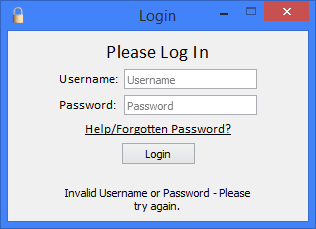
\includegraphics[width=\textwidth]{./Testing/Evidence/LoginTestFail.png}
    \caption{Test 1.1 - Invalid Login Credentials}  \label{fig:LoginTestFail}
\end{figure}

\begin{figure}[H]
    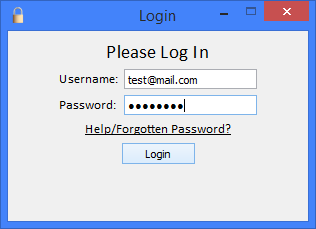
\includegraphics[width=\textwidth]{./Testing/Evidence/LoginTestSucceed.png}
    \caption{Test 1.1 - Correct Login Credentials}  \label{fig:LoginTestSucceed}
\end{figure}

\begin{figure}[H]
    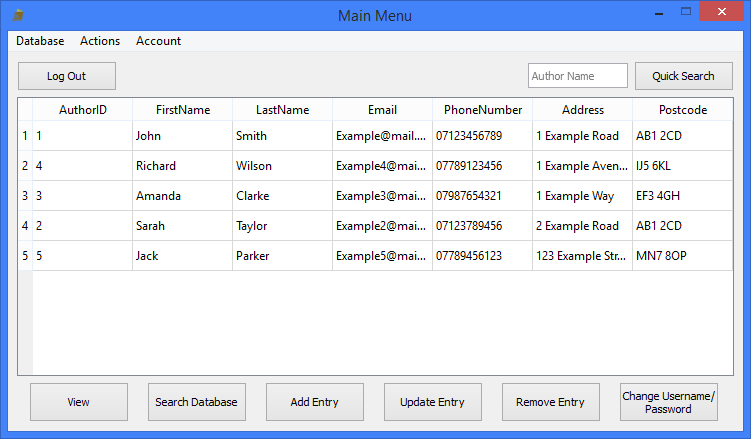
\includegraphics[width=\textwidth]{./Testing/Evidence/LoginTestSucceed2.png}
    \caption{Test 1.1 - User granted access}  \label{fig:LoginTestSucceed2}
\end{figure}

\begin{figure}[H]
    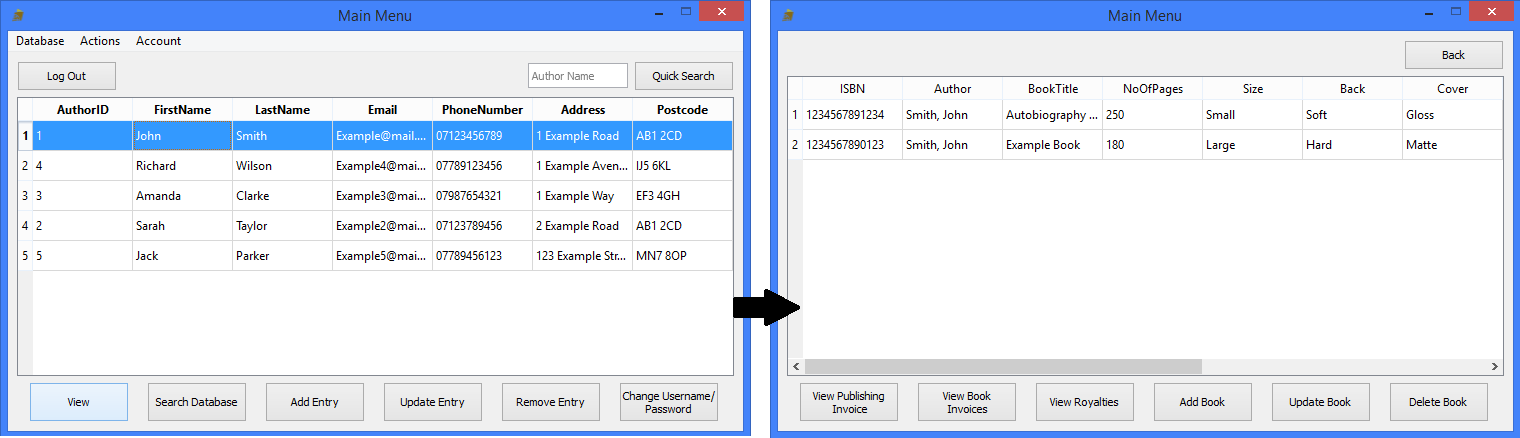
\includegraphics[width=\textwidth]{./Testing/Evidence/ViewButtonTest.png}
    \caption{Test 1.2 - Testing the View Button after selecting a customer}  \label{fig:ViewButtonTest}
\end{figure}

\begin{figure}[H]
    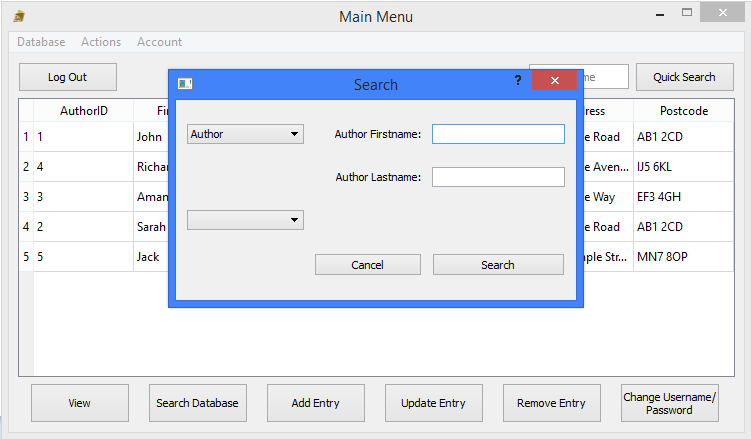
\includegraphics[width=\textwidth]{./Testing/Evidence/SearchDatabaseButtonTest.png}
    \caption{Test 1.4 - Testing the Search Database Button}  \label{fig:SearchDatabaseButtonTest}
\end{figure}

\begin{figure}[H]
    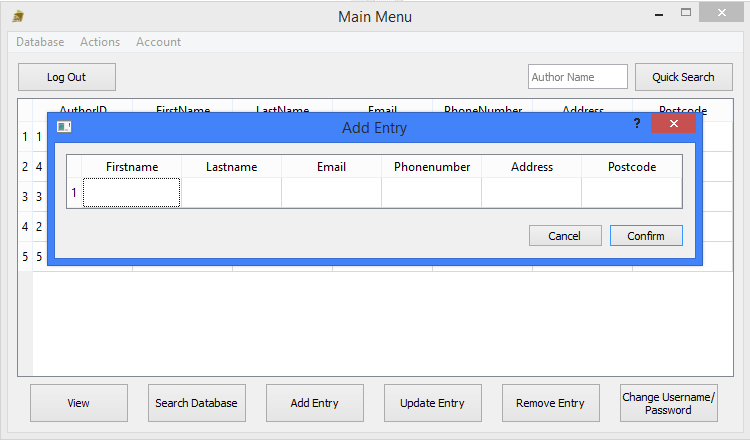
\includegraphics[width=\textwidth]{./Testing/Evidence/AddEntryButtonTest.png}
    \caption{Test 1.5 - Testing the Add Entry button}  \label{fig:AddEntryButtonTest}
\end{figure}

\begin{figure}[H]
    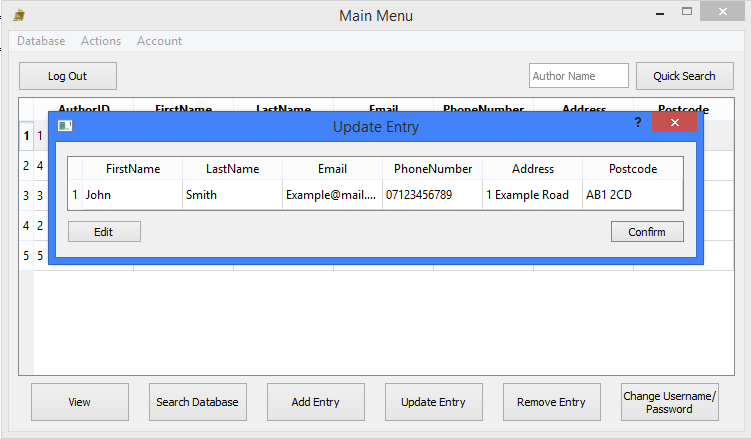
\includegraphics[width=\textwidth]{./Testing/Evidence/UpdateEntryButtonTest.png}
    \caption{Test 1.7 - Testing the Update Entry Button after selecting customer}  \label{fig:UpdateEntryButtonTest}
\end{figure}

\begin{figure}[H]
    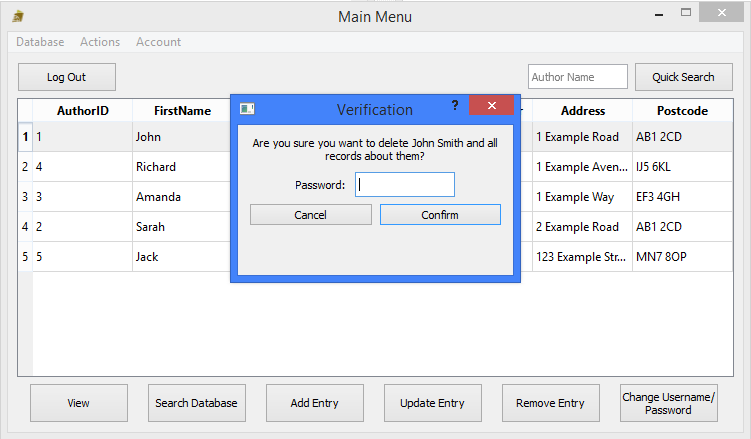
\includegraphics[width=\textwidth]{./Testing/Evidence/RemoveEntryButtonTest.png}
    \caption{Test 1.8 - Testing the Remove Entry Button after selecting a customer}  \label{fig:RemoveEntryButtonTest}
\end{figure}

\begin{figure}[H]
    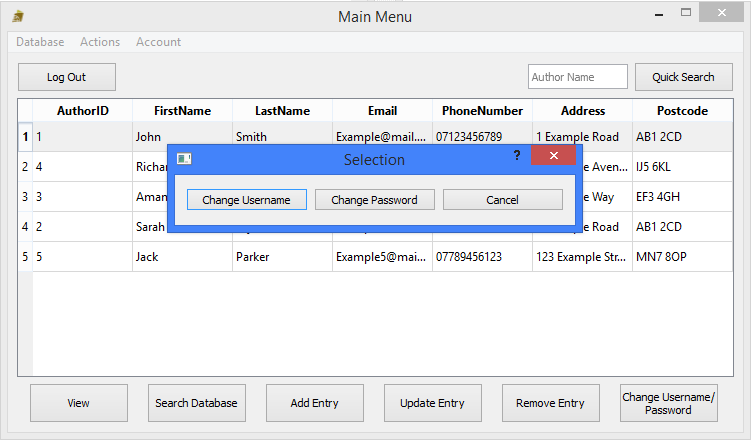
\includegraphics[width=\textwidth]{./Testing/Evidence/ChangeButtonTest.png}
    \caption{Test 1.9 - Testing the Change Username/Password Button}  \label{fig:ChangeButtonTest}
\end{figure}

\begin{figure}[H]
    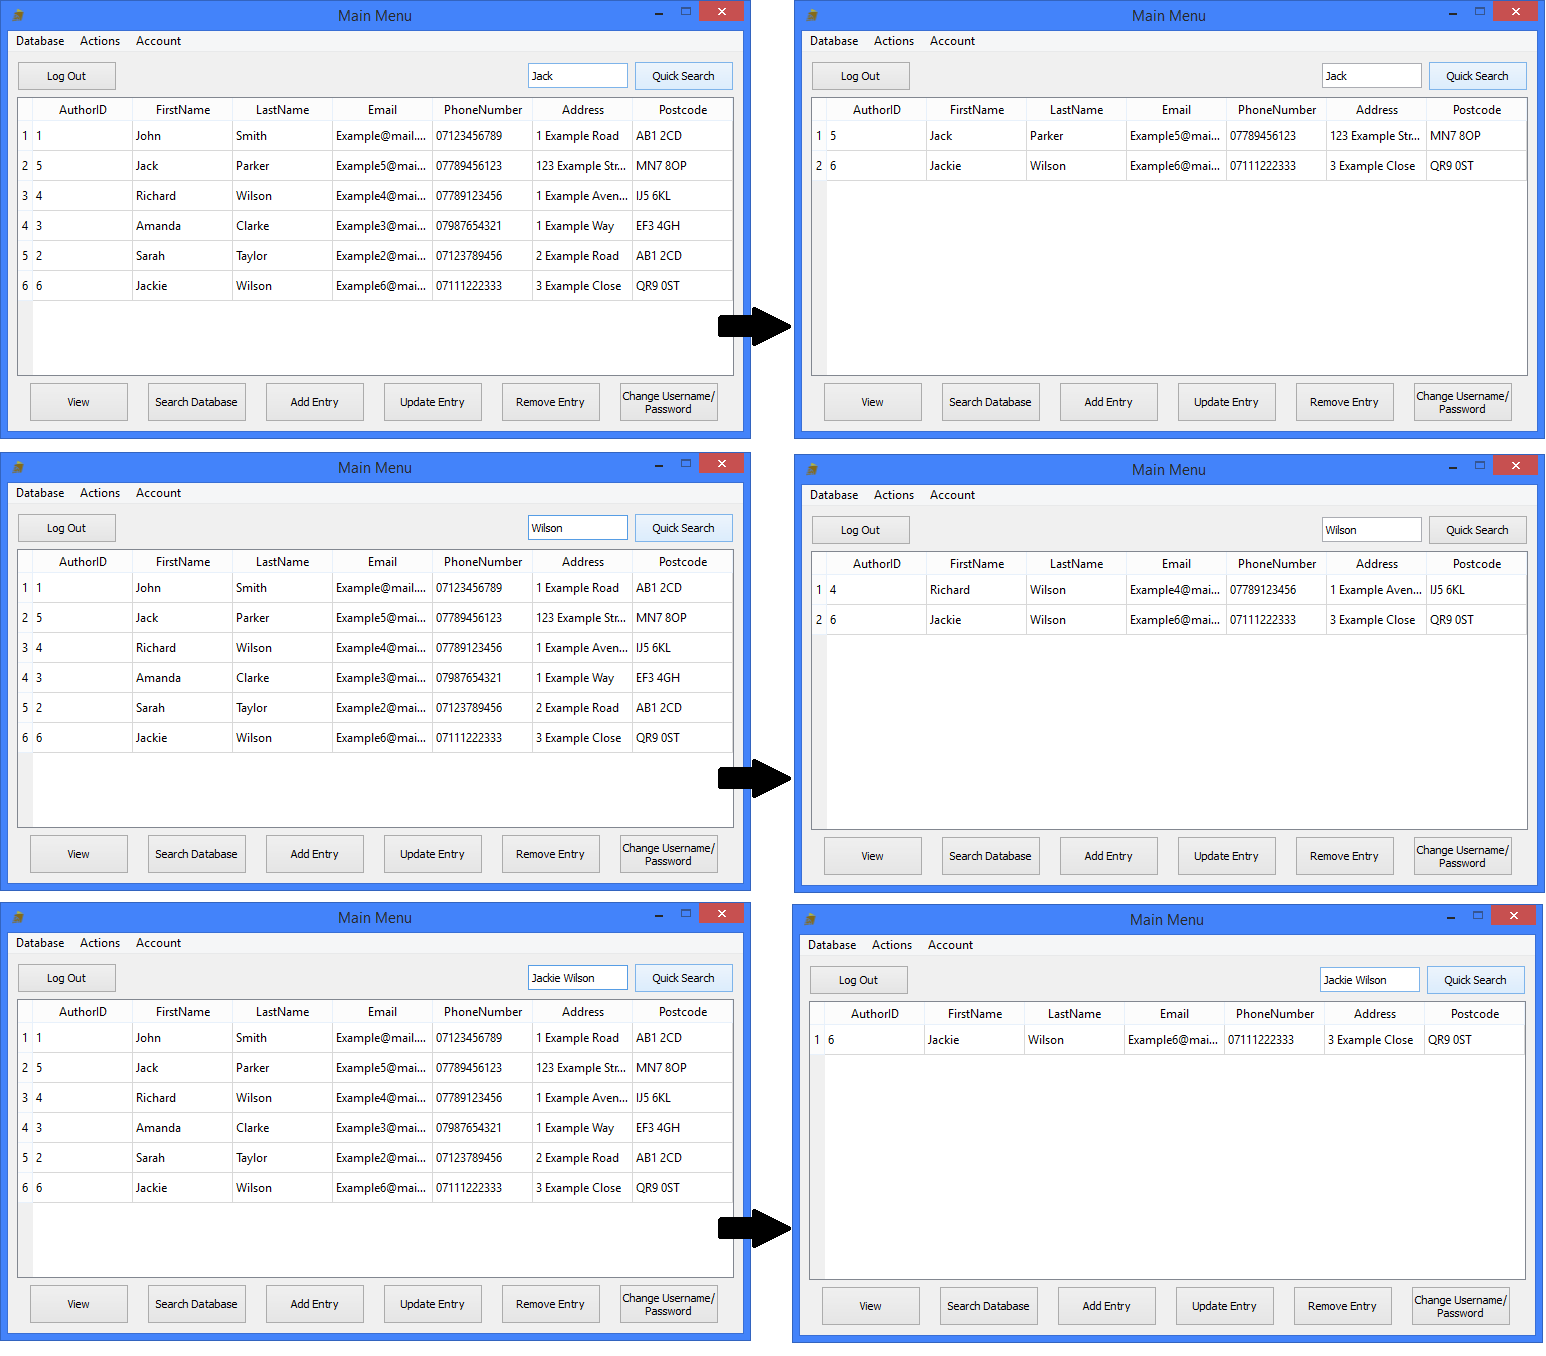
\includegraphics[width=\textwidth]{./Testing/Evidence/QuickSearchButtonTest.png}
    \caption{Test 1.10 - Testing the Quick Search Button after entering some data}  \label{fig:QuickSearchButtonTest}
\end{figure}

\begin{figure}[H]
    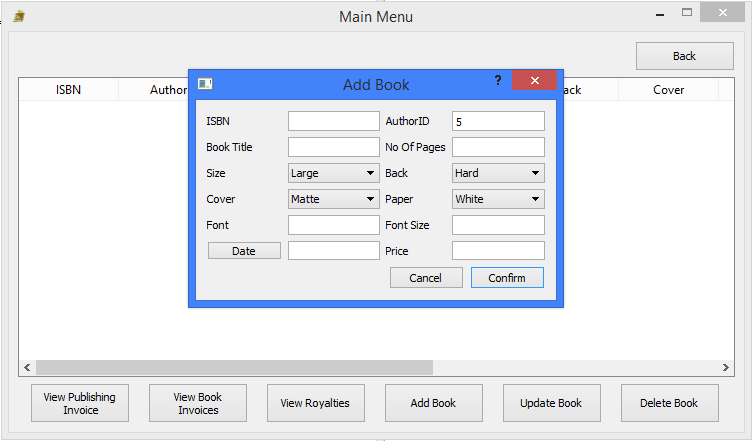
\includegraphics[width=\textwidth]{./Testing/Evidence/AddBookButtonTest.png}
    \caption{Test 1.12 - Testing the Add Book Button}  \label{fig:AddBookButtonTest}
\end{figure}

\begin{figure}[H]
    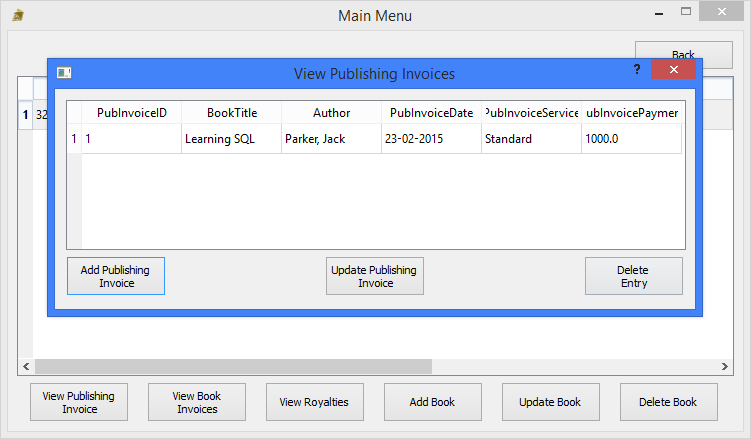
\includegraphics[width=\textwidth]{./Testing/Evidence/ViewPubInvoiceButtonTest.png}
    \caption{Test 1.13 - Testing the View Publishing Invoice Button after selecting a book}  \label{fig:ViewPubInvoiceButtonTest}
\end{figure}

\begin{figure}[H]
    \includegraphics[width=\textwidth]{./Testing/Evidence/{ViewRoyaltiesButtonTest}.png}
    \caption{Test 1.14 - Testing the View Royalties Button after selecting a book}  \label{fig:ViewRoyaltiesButtonTest}
\end{figure}

\begin{figure}[H]
    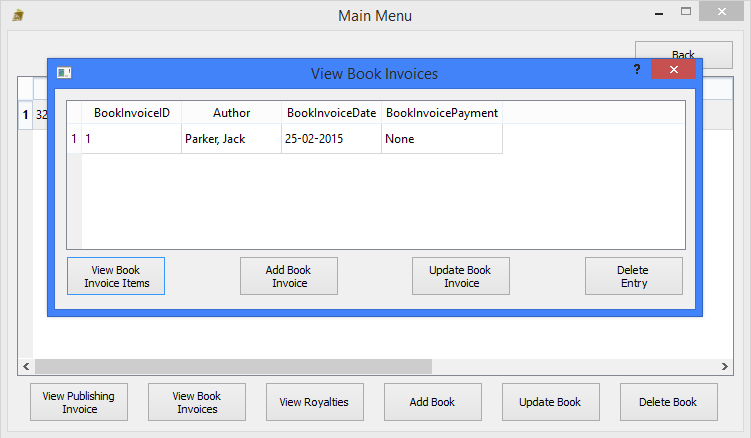
\includegraphics[width=\textwidth]{./Testing/Evidence/ViewBookInvoiceButtonTest.png}
    \caption{Test 1.15 - Testing the View Book Invoice Button after selecting a book}  \label{fig:ViewBookInvoiceButtonTest}
\end{figure}

\begin{figure}[H]
    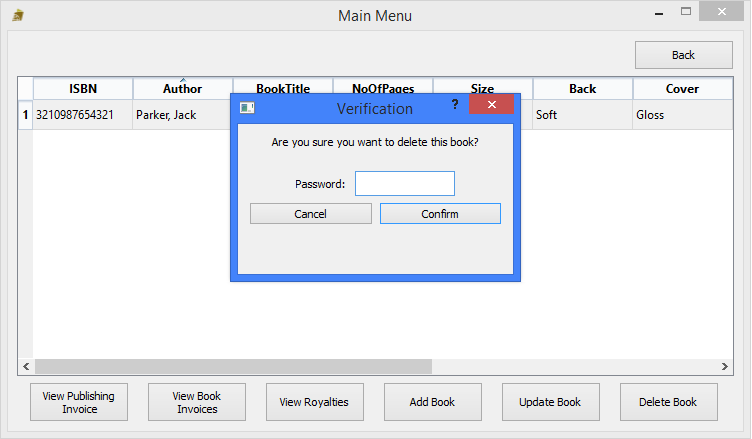
\includegraphics[width=\textwidth]{./Testing/Evidence/DeleteBookButtonTest.png}
    \caption{Test 1.16 - Testing the Delete Book Button after selecting a book}  \label{fig:DeleteBookButtonTest}
\end{figure}

\begin{figure}[H]
    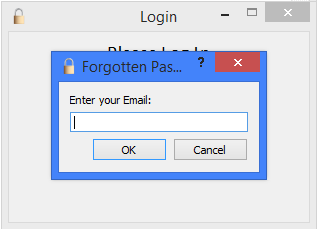
\includegraphics[width=\textwidth]{./Testing/Evidence/ForgotPasswordLabelTest.png}
    \caption{Test 1.17  - Testing the Forgot Password label on the login screen}  \label{fig:ForgotPasswordLabelTest}
\end{figure}

\begin{figure}[H]
    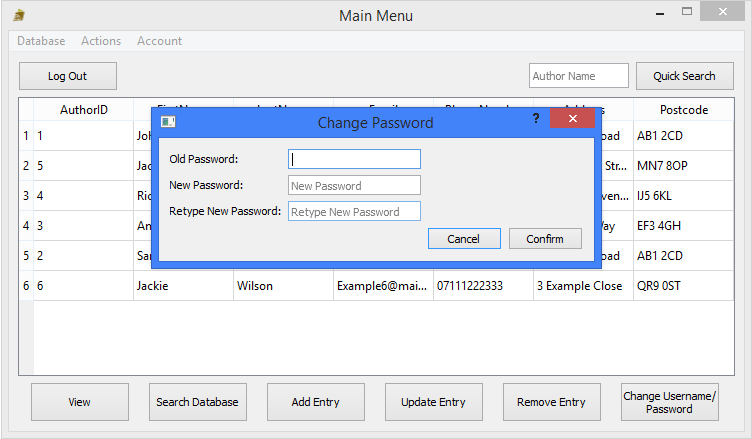
\includegraphics[width=\textwidth]{./Testing/Evidence/ChangePasswordButtonTest.png}
    \caption{Test 1.18 - Testing the Change Password button}  \label{fig:ChangePasswordButtonTest}
\end{figure}

\begin{figure}[H]
    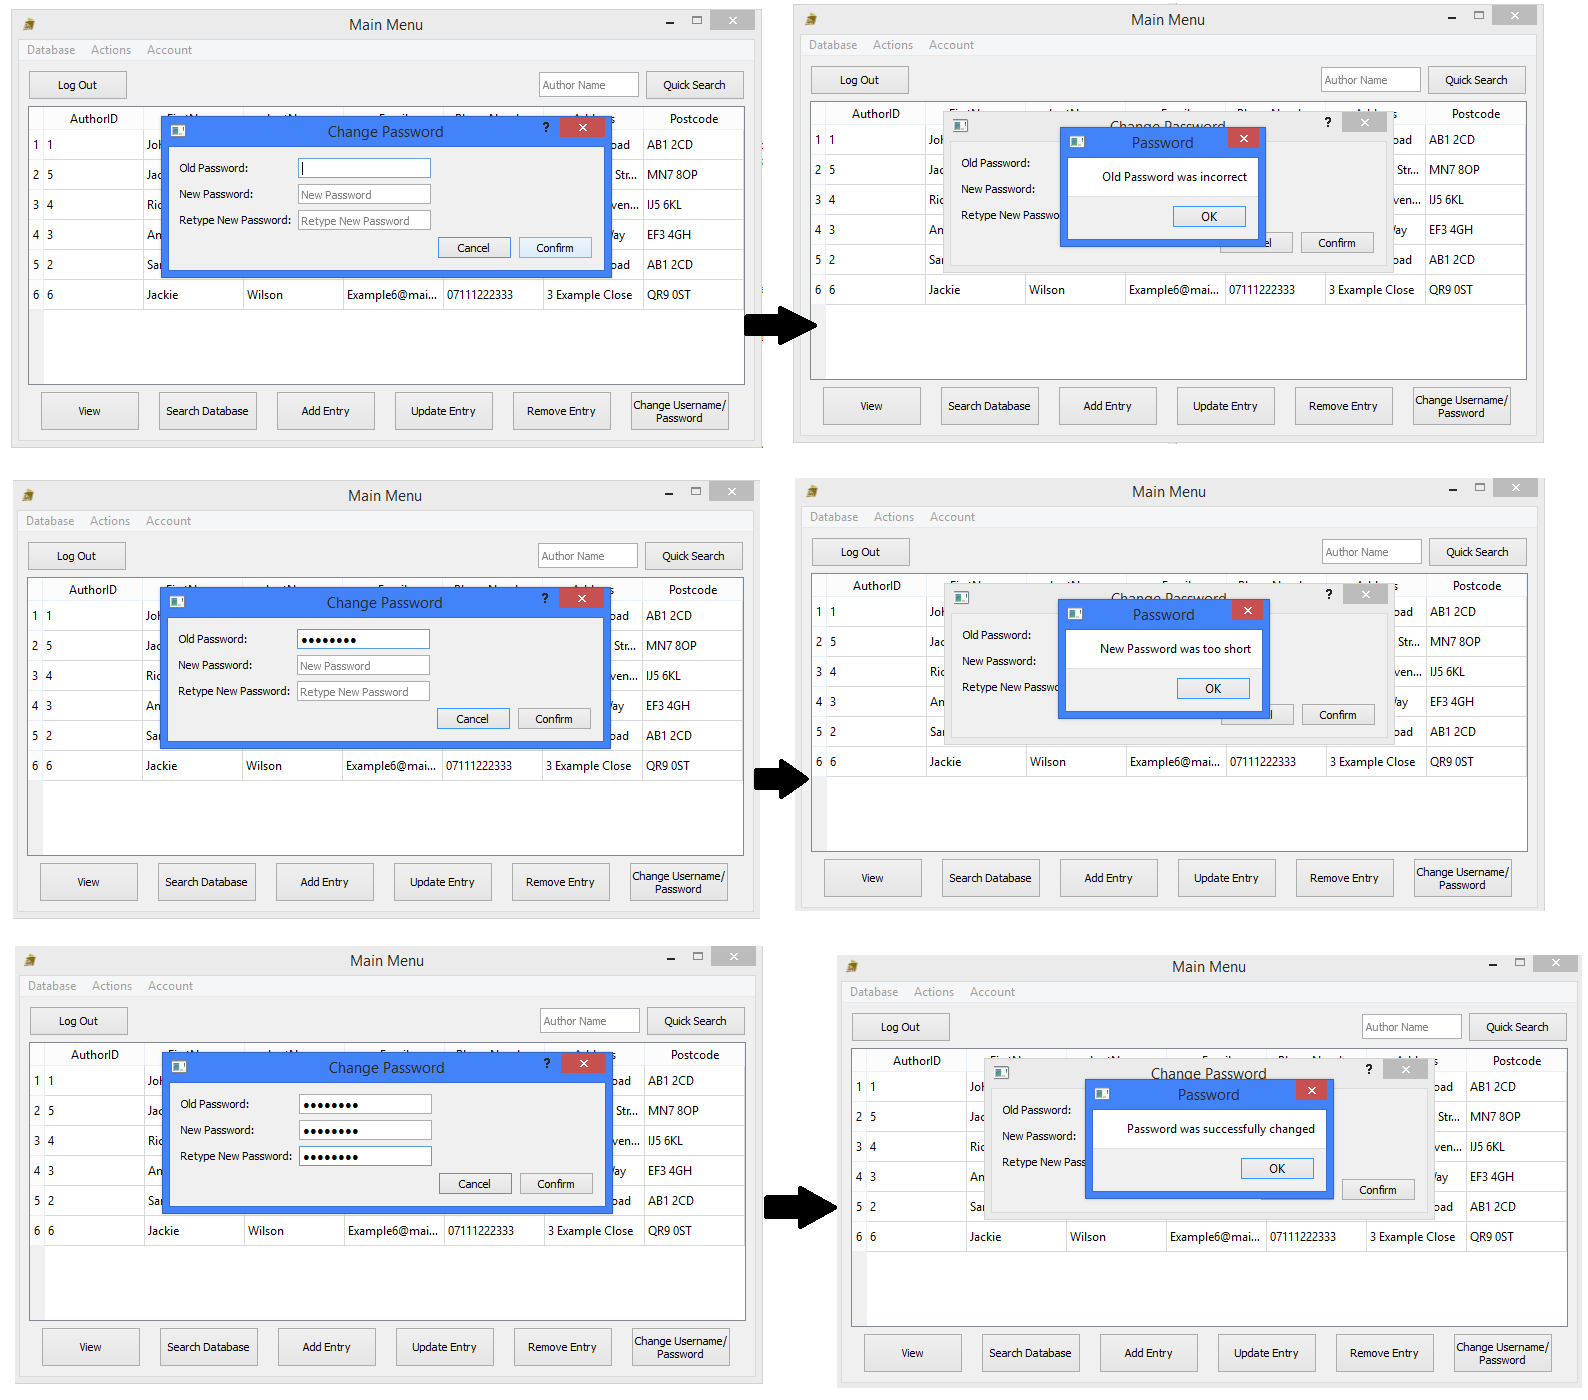
\includegraphics[width=\textwidth]{./Testing/Evidence/ConfirmPasswordButtonTest.png}
    \caption{Test 1.19 - Testing the Confirm button after entering new password details}  \label{fig:ConfirmPasswordButtonTest}
\end{figure}

\begin{figure}[H]
    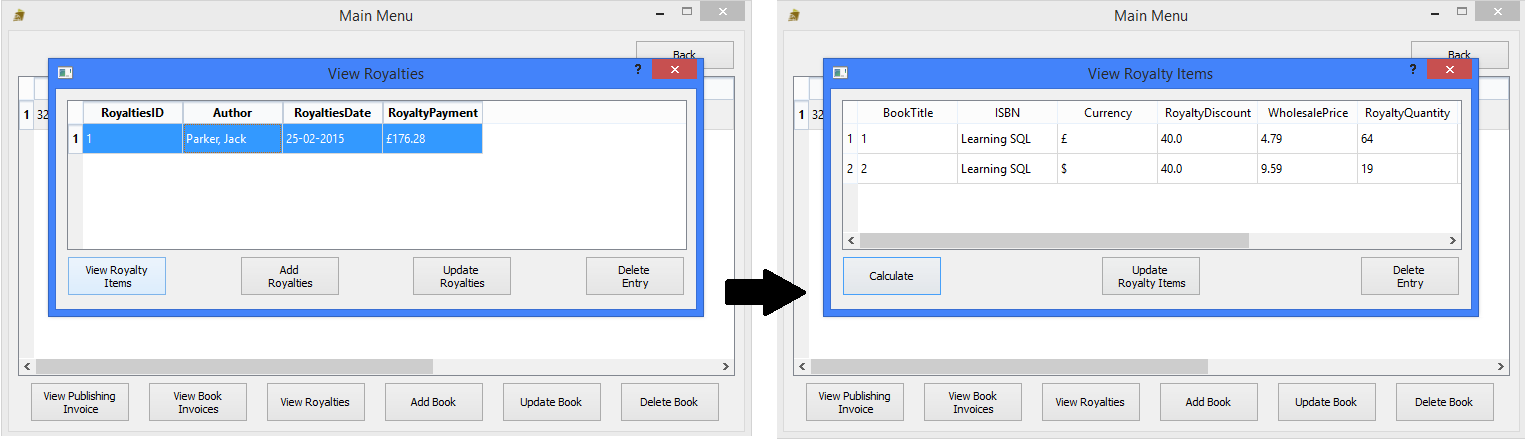
\includegraphics[width=\textwidth]{./Testing/Evidence/ViewRoyaltyItemsButtonTest.png}
    \caption{Test 1.20 - Testing the View Royalty Items button after selecting a Royalty payment}  \label{fig:ViewRoyaltyItemsButtonTest}
\end{figure}

\begin{figure}[H]
    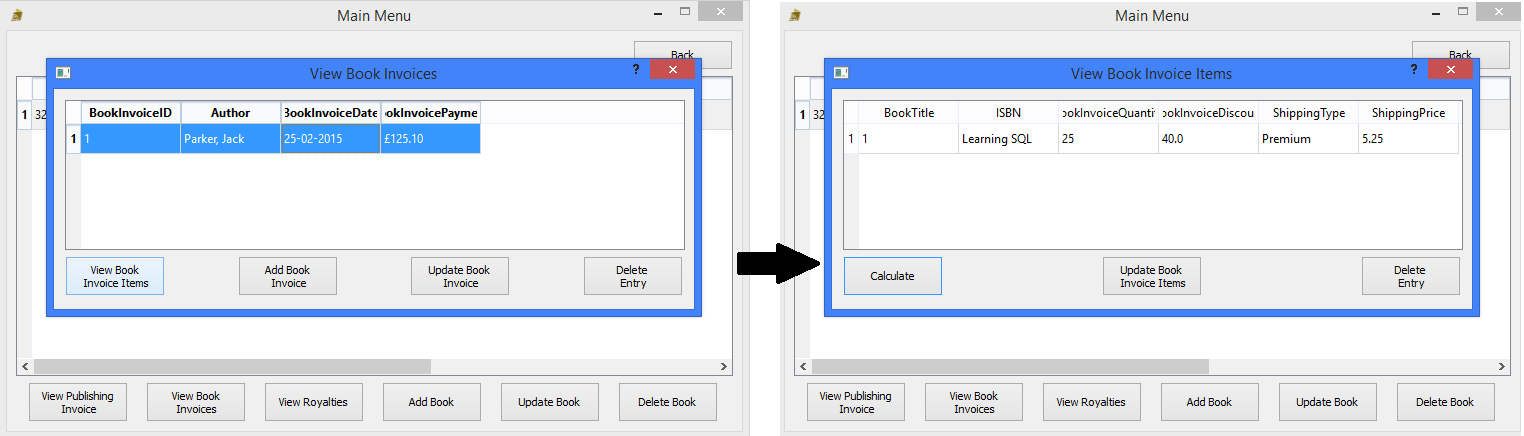
\includegraphics[width=\textwidth]{./Testing/Evidence/ViewBookInvoiceItemsButtonTest.png}
    \caption{Test 1.21 - Testing the View Book Invoice Items button after selecting a Book Invoice}  \label{fig:ViewBookInvoiceItemsButtonTest}
\end{figure}

\begin{figure}[H]
    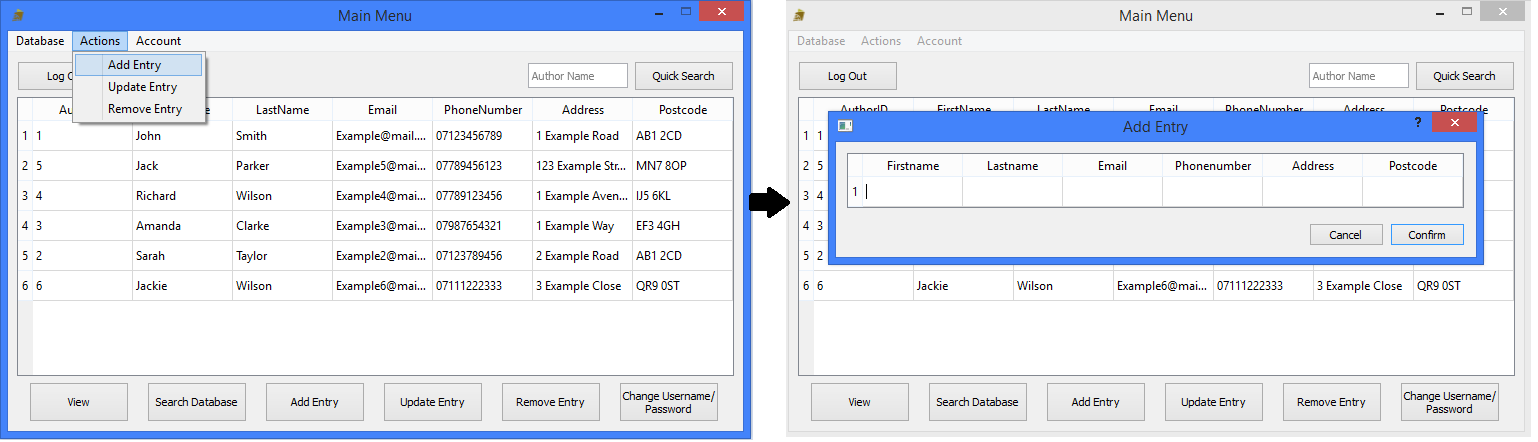
\includegraphics[width=\textwidth]{./Testing/Evidence/AddEntryMenuTest.png}
    \caption{Test 1.23 - Testing the Add Entry option on the menu bar}  \label{fig:AddEntryMenuTest}
\end{figure}

\begin{figure}[H]
    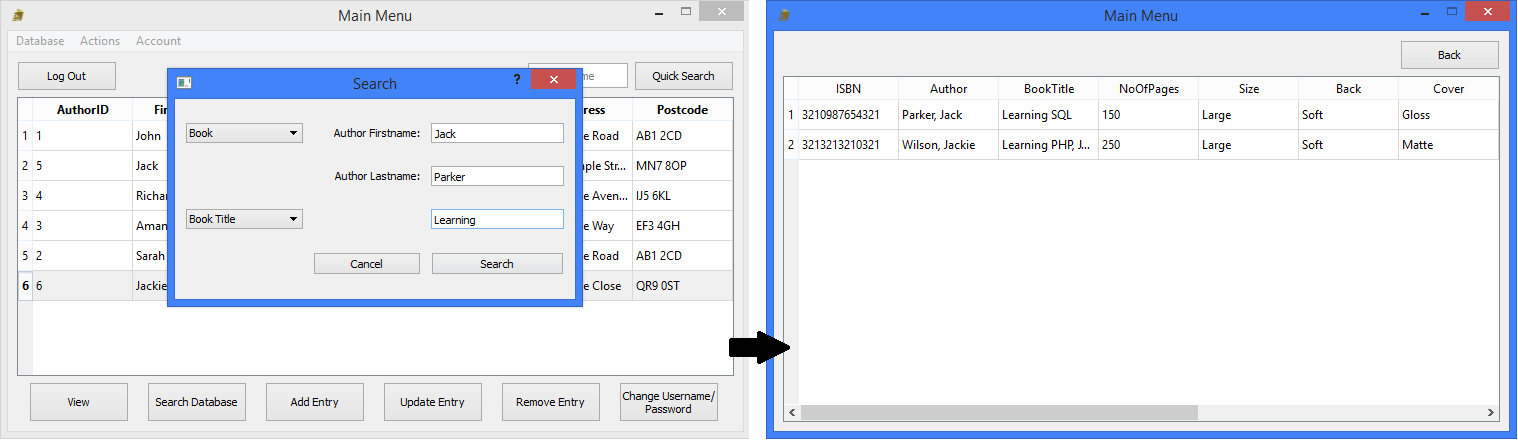
\includegraphics[width=\textwidth]{./Testing/Evidence/ConfirmSearchButtonTest.png}
    \caption{Test 1.24 - Testing the Confirm button on the search window after having entered some data}  \label{fig:ConfirmSearchButtonTest}
\end{figure}

\begin{figure}[H]
    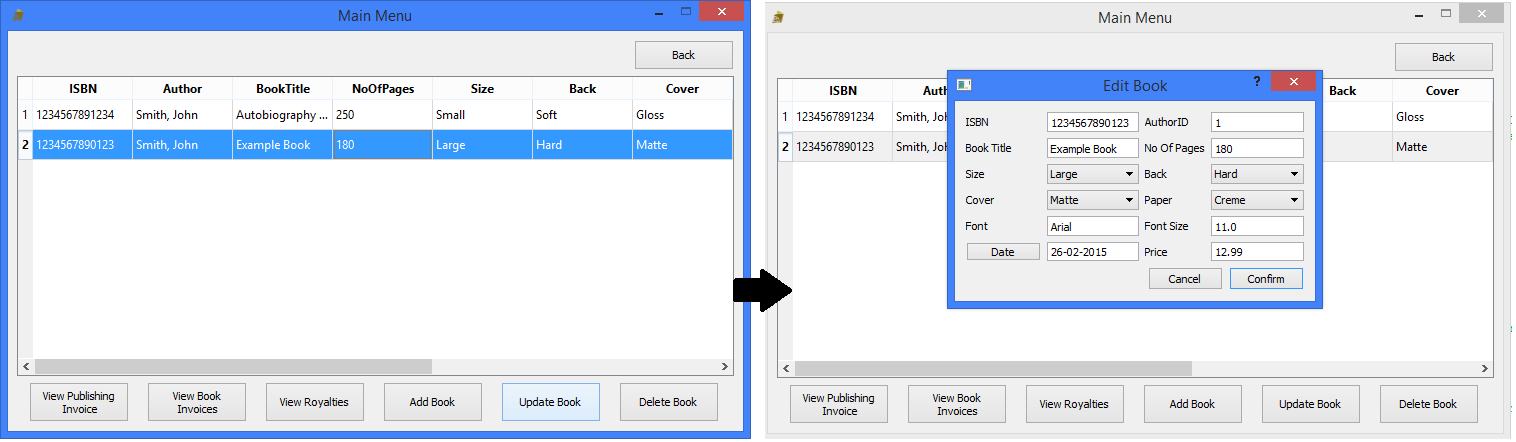
\includegraphics[width=\textwidth]{./Testing/Evidence/UpdateBookButtonTest.png}
    \caption{Test 1.27 - Testing the Update Book button after selecting a book}  \label{fig:UpdateBookButtonTest}
\end{figure}

\begin{figure}[H]
    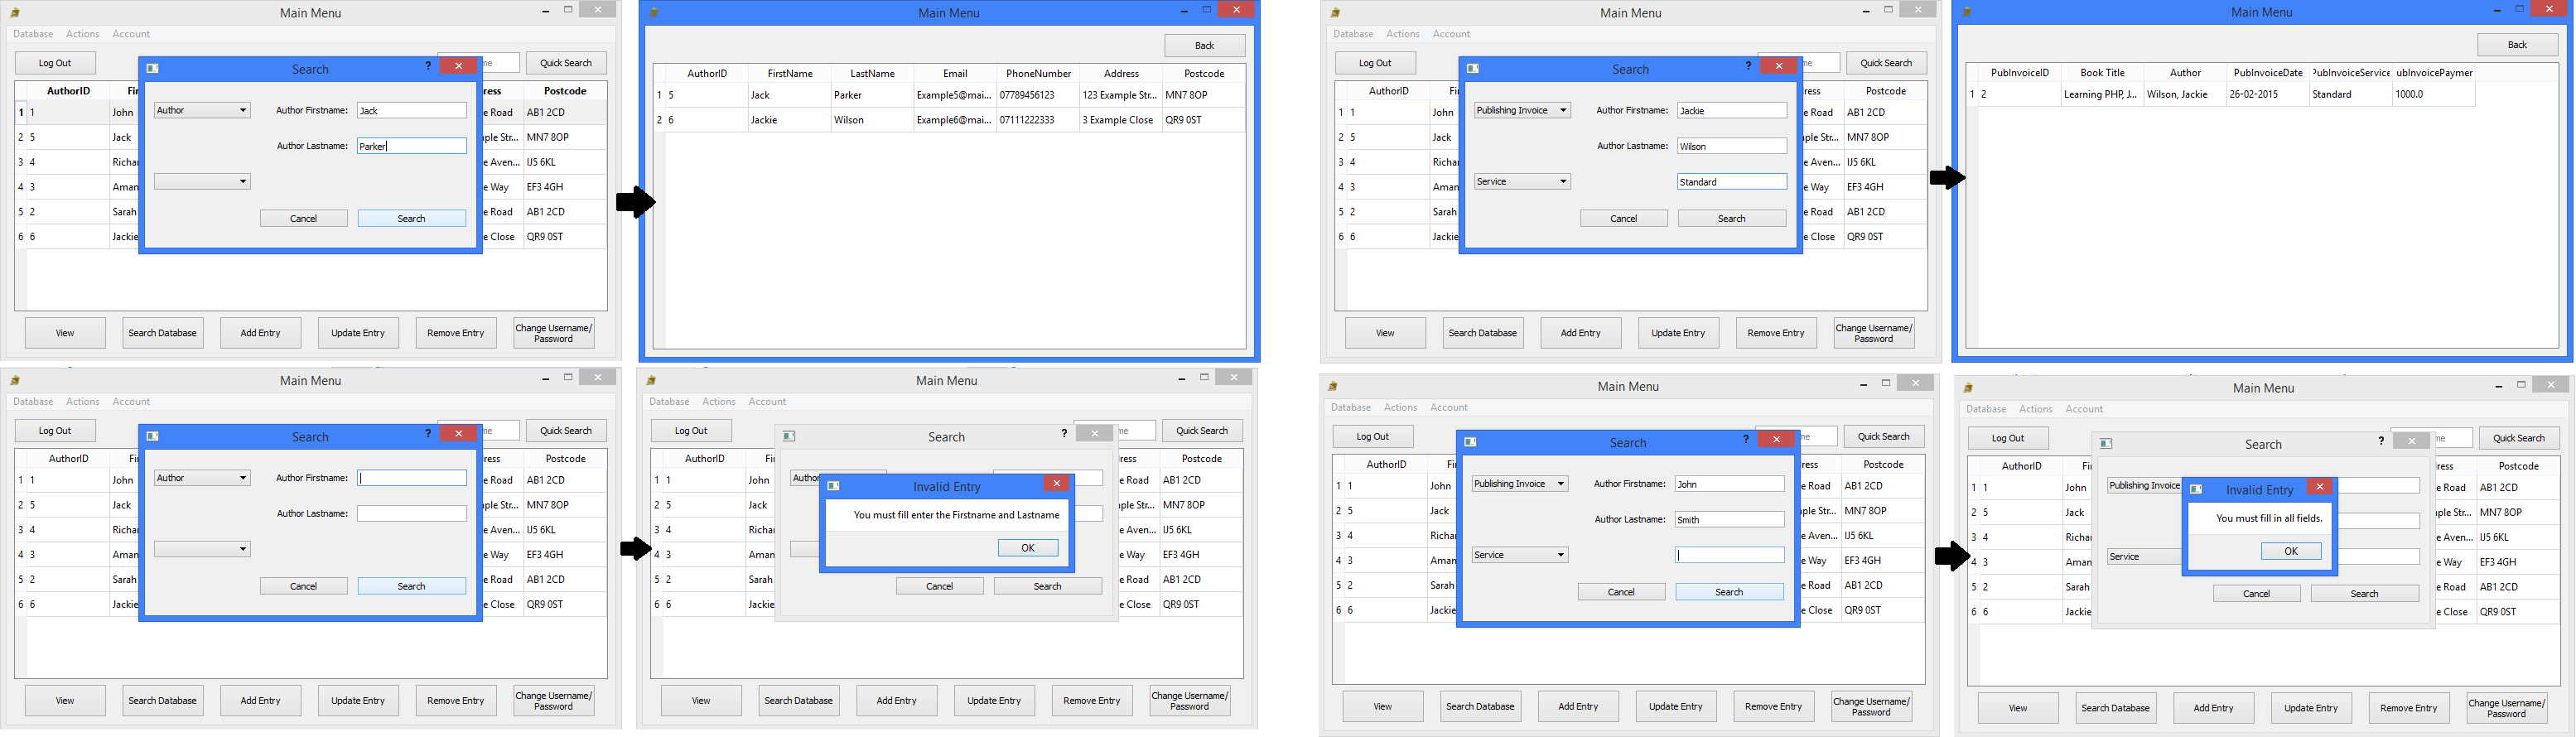
\includegraphics[width=\textwidth]{./Testing/Evidence/Series2/SearchValidation.png}
    \caption{Test 2.1 - Validation for inputs in the search window}  \label{fig:SearchValidation}
\end{figure}

\begin{figure}[H]
    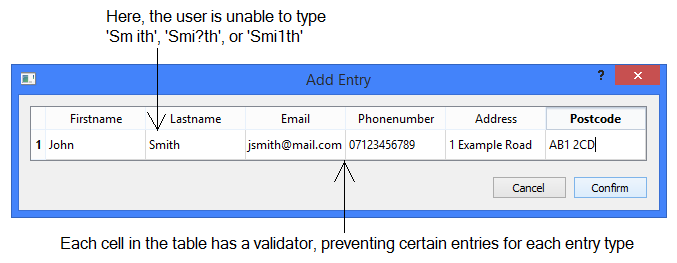
\includegraphics[width=\textwidth]{./Testing/Evidence/Series2/AddEntryValidation.png}
    \caption{Test 2.3, 2.4, 2.5, 2.6 - Validation for adding customer details}  \label{fig:AddEntryValidation}
\end{figure}

\begin{figure}[H]
    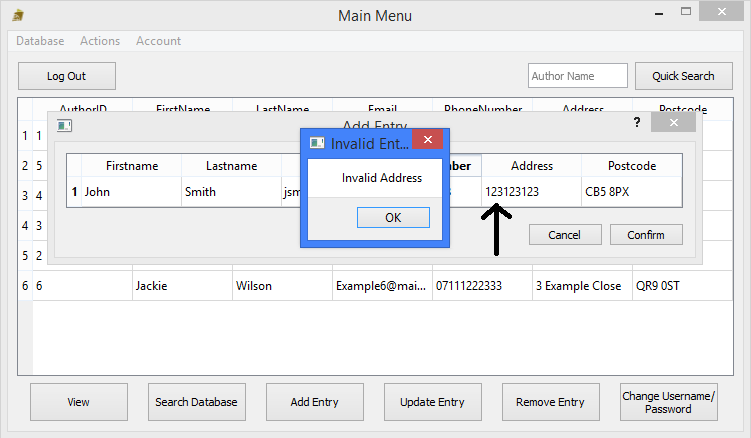
\includegraphics[width=\textwidth]{./Testing/Evidence/Series2/InvalidAddress.png}
    \caption{Test 2.6 - Prompting the user with an error when an invalid address has been entered}  \label{fig:InvalidAddress}
\end{figure}

\begin{figure}[H]
    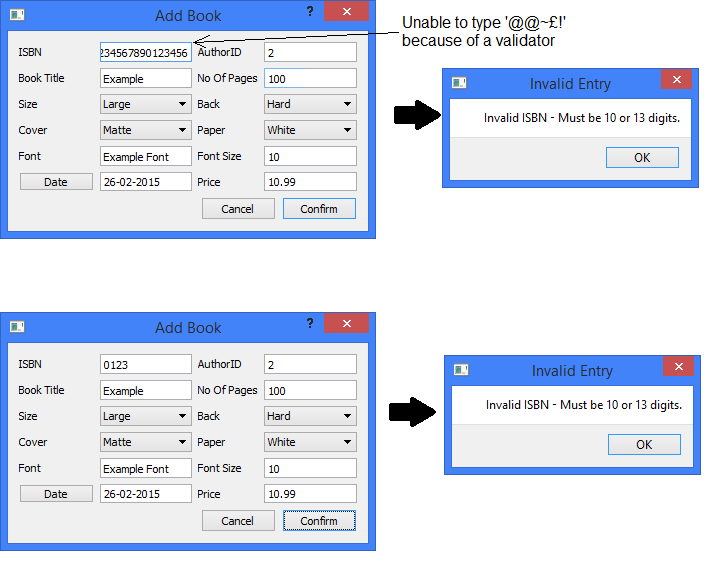
\includegraphics[width=\textwidth]{./Testing/Evidence/Series2/ISBNRejection.png}
    \caption{Test 2.7 - Validating the ISBN}  \label{fig:ISBNRejection}
\end{figure}

\begin{figure}[H]
    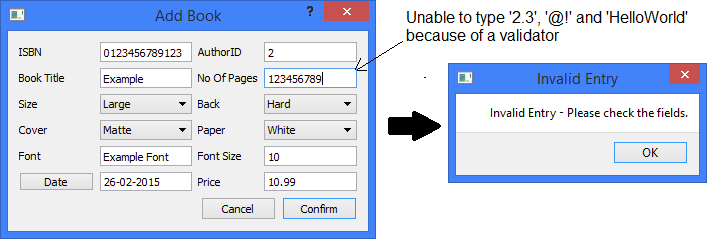
\includegraphics[width=\textwidth]{./Testing/Evidence/Series2/PagesRejection.png}
    \caption{Test 2.8 - Validating the No of pages entered}  \label{fig:PagesRejection}
\end{figure}

\begin{figure}[H]
    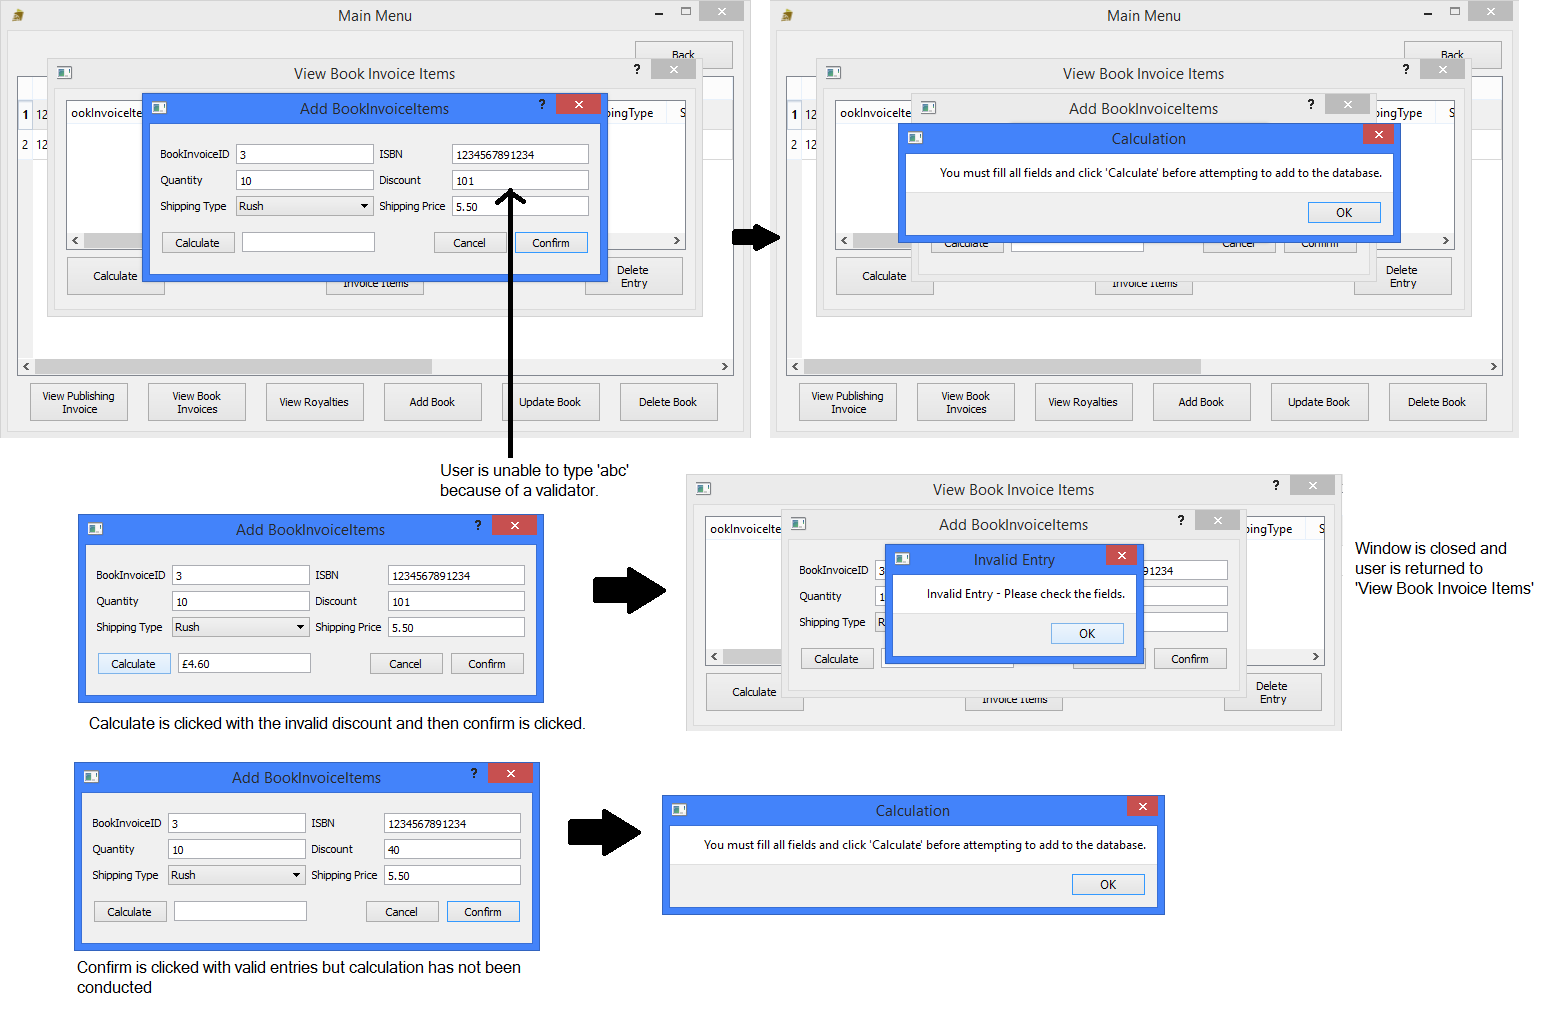
\includegraphics[width=\textwidth]{./Testing/Evidence/Series2/BookInvoiceDiscountValidation.png}
    \caption{Test 2.9 -  Validating the Discount when adding Book Invoice Items}  \label{fig:BookInvoiceDiscountValidation}
\end{figure}

\begin{figure}[H]
    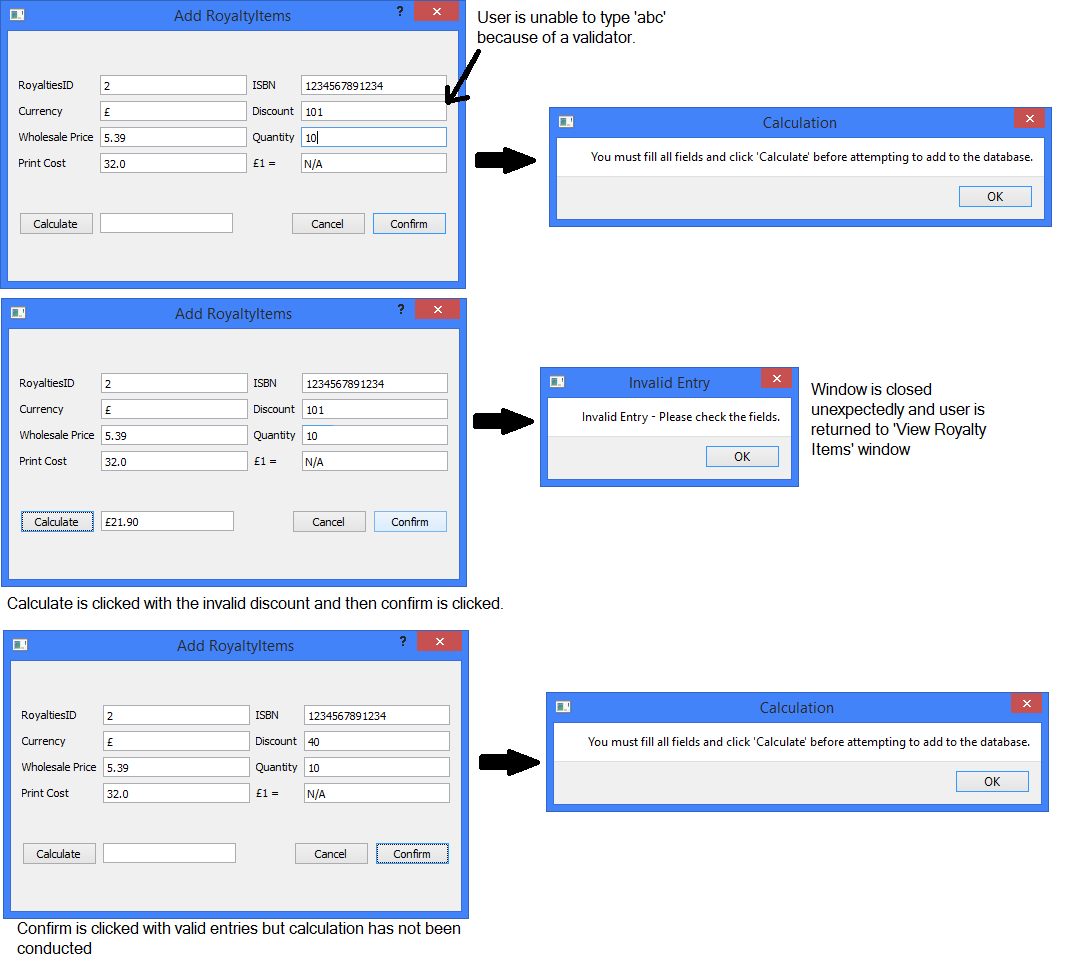
\includegraphics[width=\textwidth]{./Testing/Evidence/Series2/RoyaltyDiscountValidation.png}
    \caption{Test 2.10 -  Validating the Discount when adding Royalty Items}  \label{fig:RoyaltyDiscountValidation}
\end{figure}

\begin{figure}[H]
    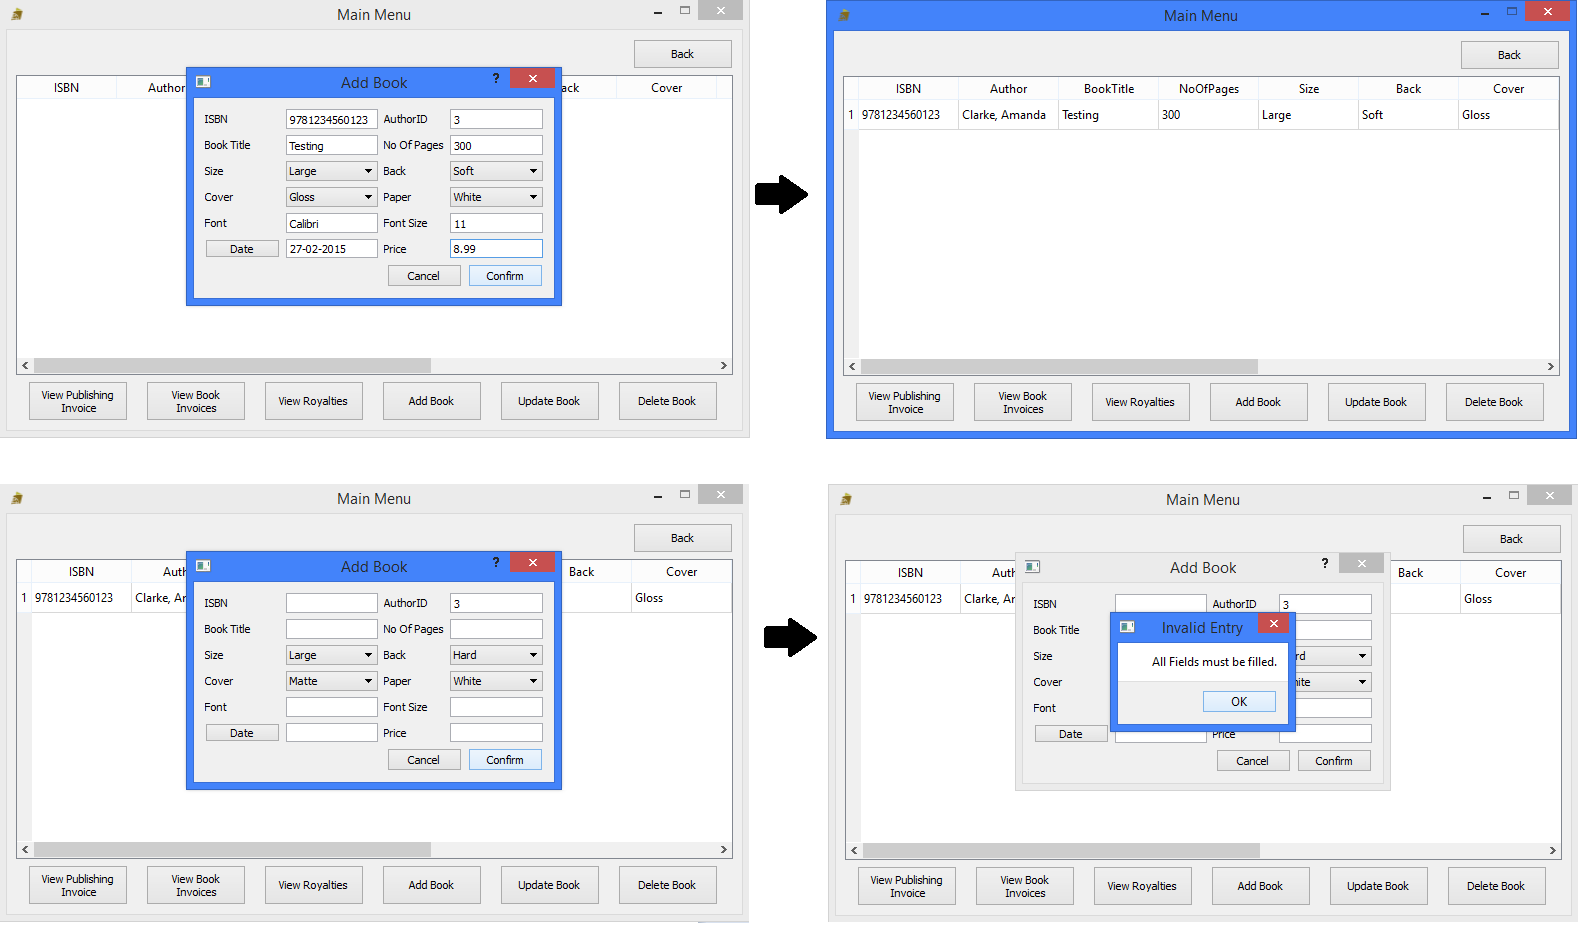
\includegraphics[width=\textwidth]{./Testing/Evidence/Series3/AddBookValidation.png}
    \caption{Test 3.1 - Adding a book}  \label{fig:AddBookValidation}
\end{figure}

\begin{figure}[H]
    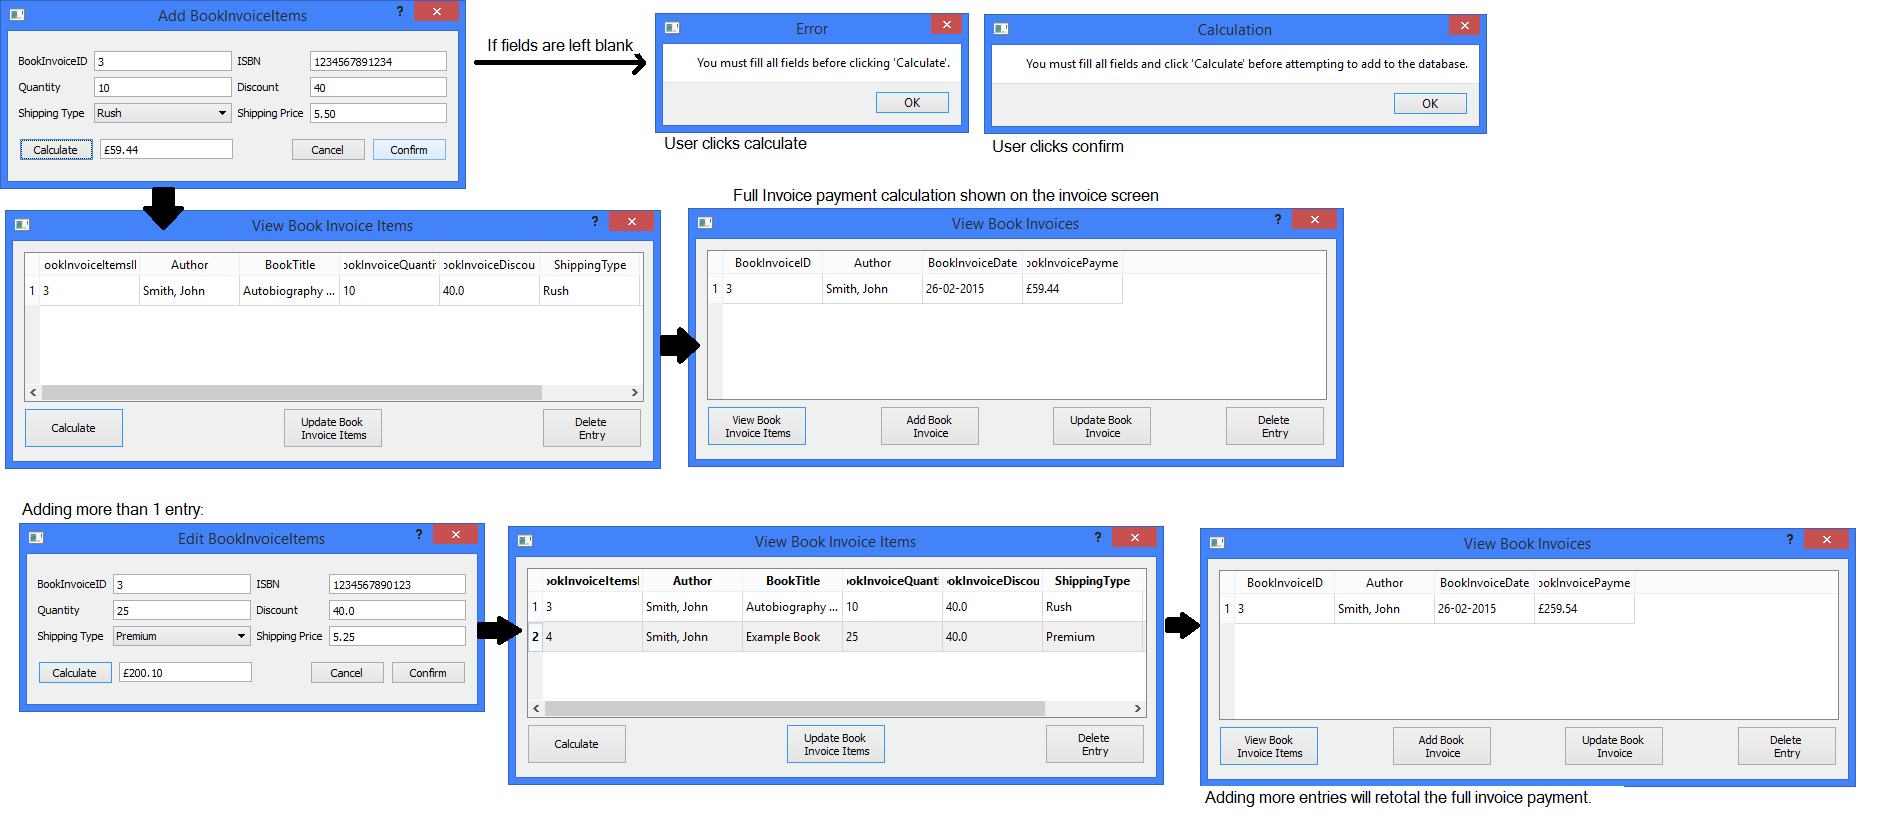
\includegraphics[width=\textwidth]{./Testing/Evidence/Series3/AddInvoiceItemTest.png}
    \caption{Test 3.2 - Calculations for adding Book Invoice items}  \label{fig:AddInvoiceItemTest}
\end{figure}

\begin{figure}[H]
    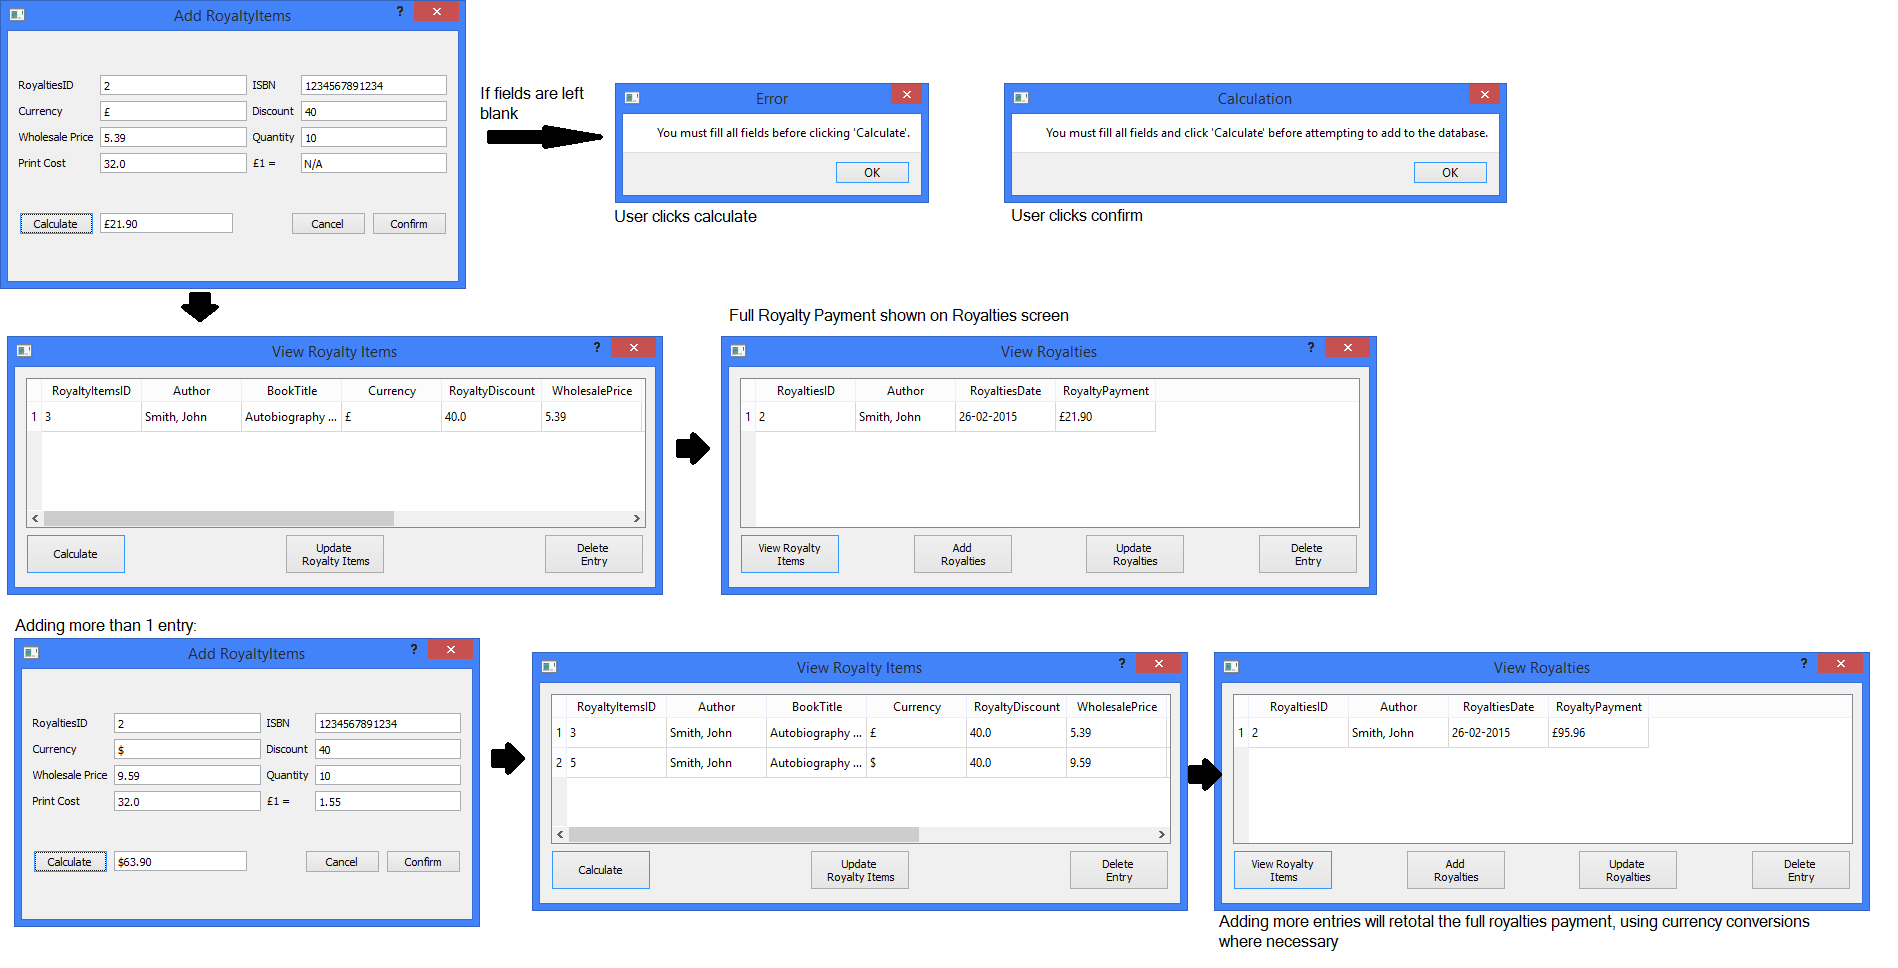
\includegraphics[width=\textwidth]{./Testing/Evidence/Series3/AddRoyaltyItemTest.png}
    \caption{Test 3.3 - Calculations for adding Royalty Items}  \label{fig:AddRoyaltyItemTest}
\end{figure}

\begin{figure}[H]
    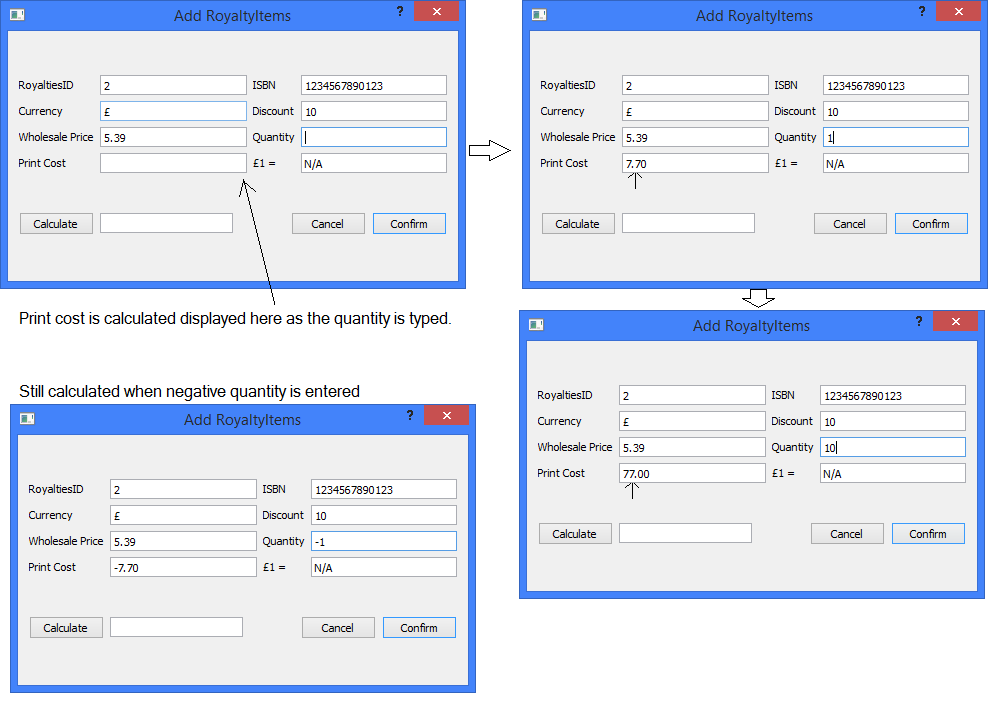
\includegraphics[width=\textwidth]{./Testing/Evidence/Series3/PrintCostValidation.png}
    \caption{Test 3.4 - Testing values for Calculating Print cost}  \label{fig:PrintCostValidation}
\end{figure}

\begin{figure}[H]
    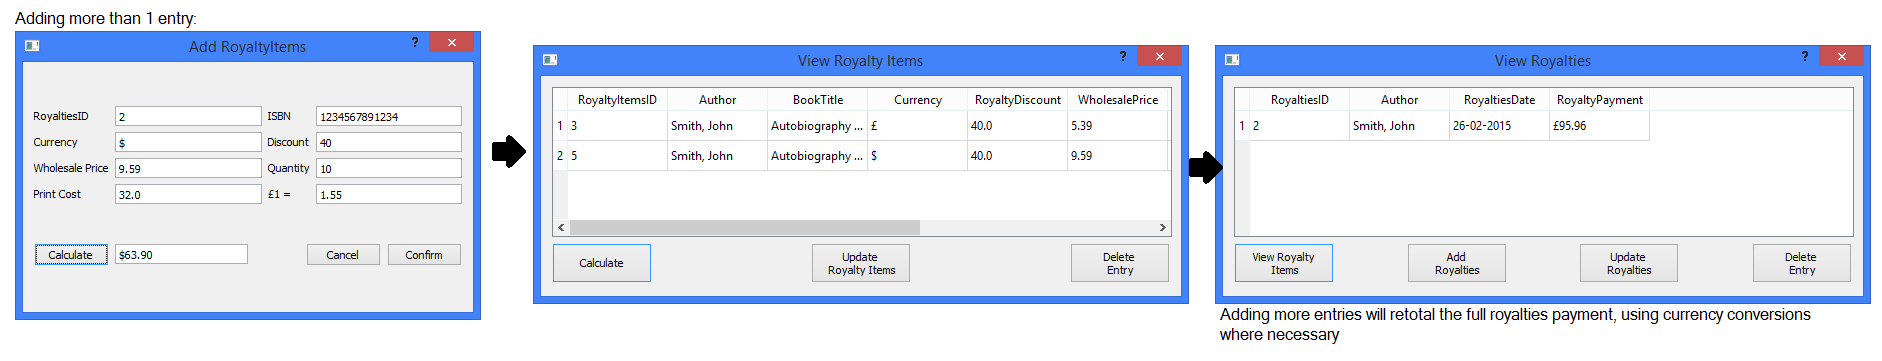
\includegraphics[width=\textwidth]{./Testing/Evidence/Series3/RoyaltyPaymentValidation.png}
    \caption{Test 3.5 - Calculating the Royalty Payment}  \label{fig:RoyaltyPaymentValidation}
\end{figure}

\begin{figure}[H]
    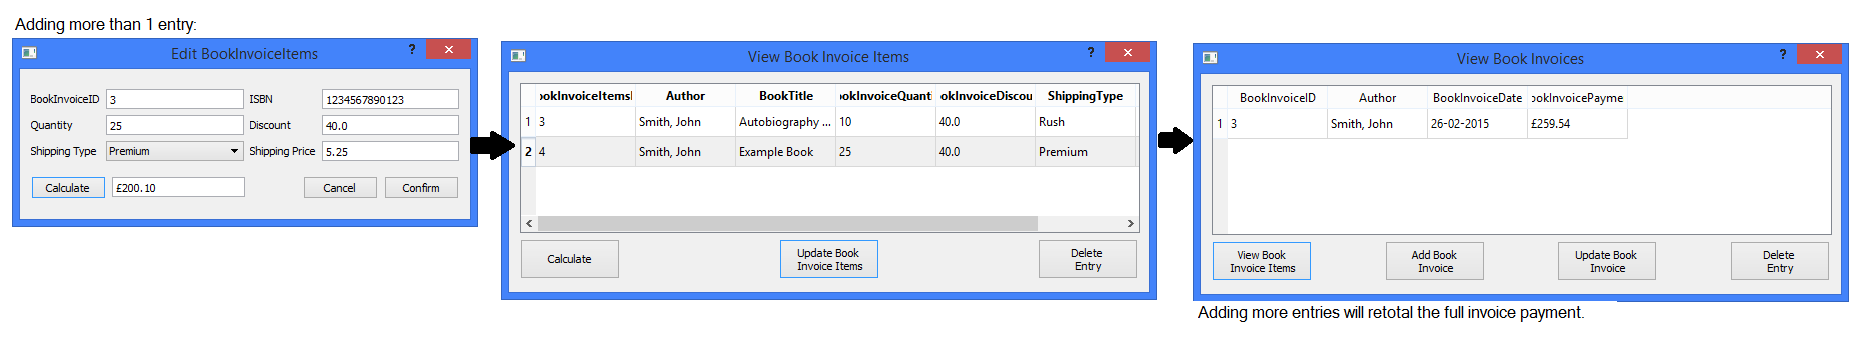
\includegraphics[width=\textwidth]{./Testing/Evidence/Series3/BookInvoicePaymentValidation.png}
    \caption{Test 3.6 - Calculating the Book Invoice Payment}  \label{fig:BookInvoicePaymentValidation}
\end{figure}

\begin{figure}[H]
    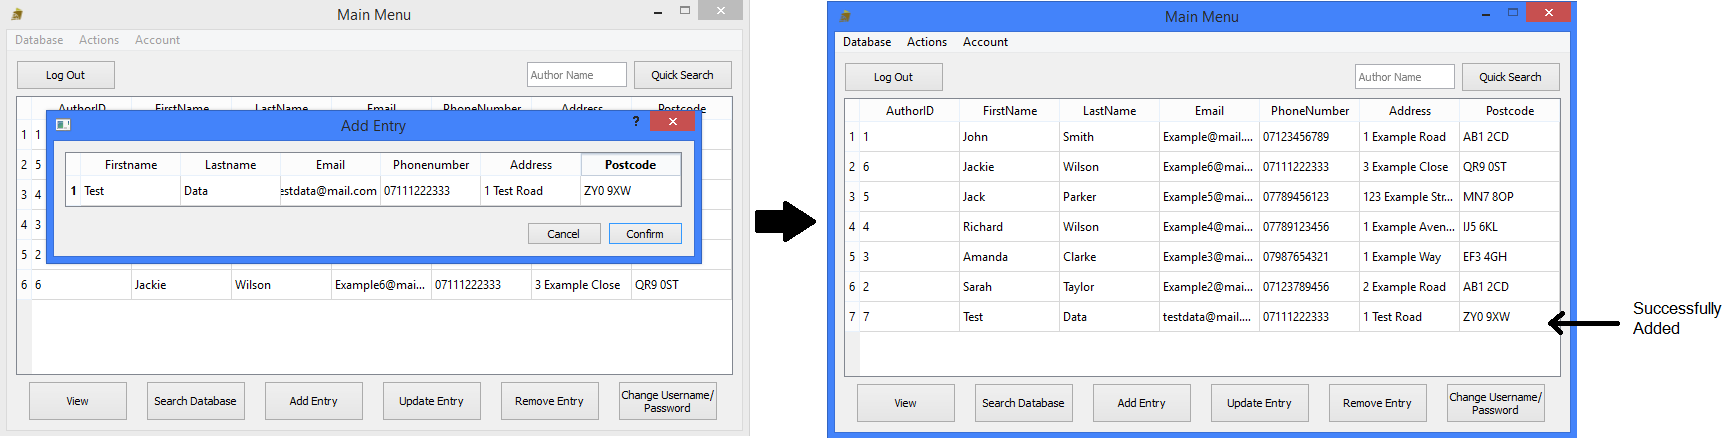
\includegraphics[width=\textwidth]{./Testing/Evidence/Series4/AddAuthorTest.png}
    \caption{Test 4.1 - Testing the process of adding an author}  \label{fig:AddAuthorTest}
\end{figure}

\begin{figure}[H]
    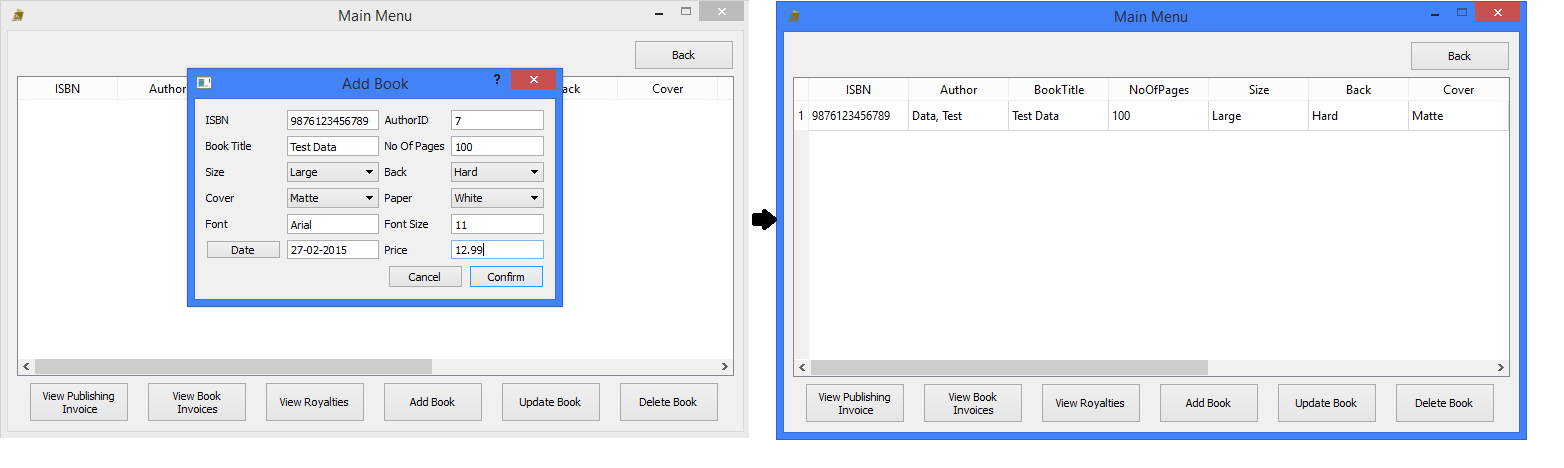
\includegraphics[width=\textwidth]{./Testing/Evidence/Series4/AddBookTest.png}
    \caption{Test 4.2 - Testing the process of adding a book}  \label{fig:AddBookTest}
\end{figure}

\begin{figure}[H]
    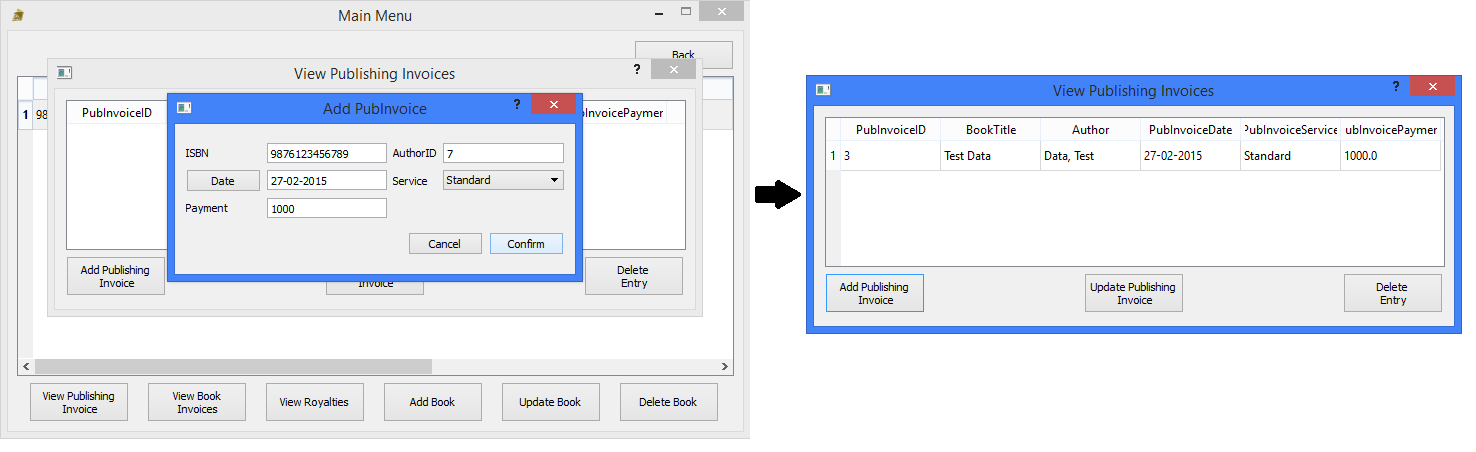
\includegraphics[width=\textwidth]{./Testing/Evidence/Series4/AddPubInvoiceTest.png}
    \caption{Test 4.3 - Testing the process of adding a Publishing Invoice}  \label{fig:AddPubInvoiceTest}
\end{figure}

\begin{figure}[H]
    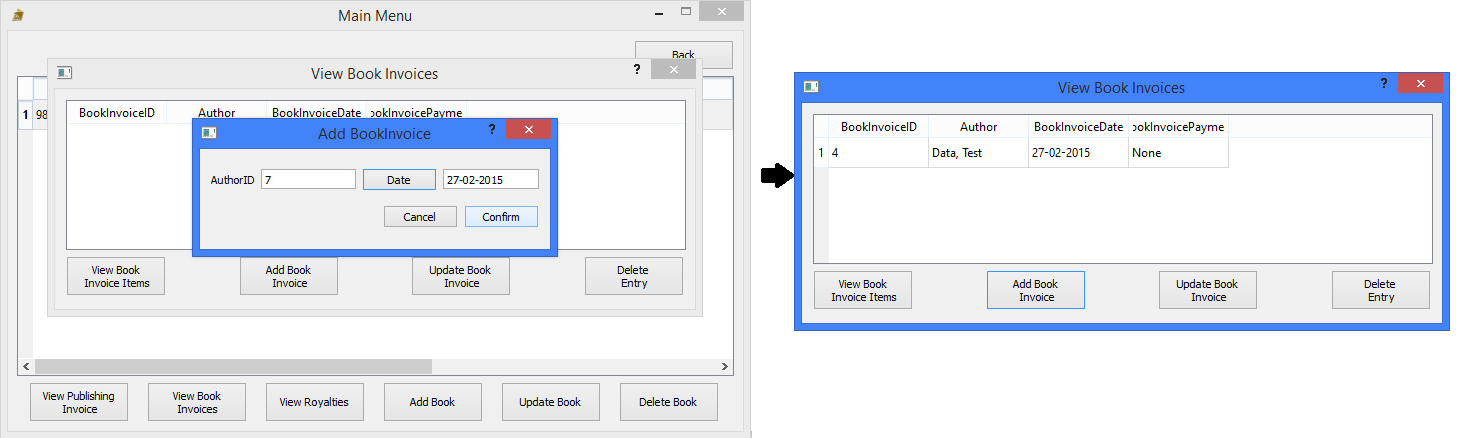
\includegraphics[width=\textwidth]{./Testing/Evidence/Series4/AddBookInvoiceTest.png}
    \caption{Test 4.4 - Testing the process of adding a Book Invoice}  \label{fig:AddBookInvoiceTest}
\end{figure}

\begin{figure}[H]
    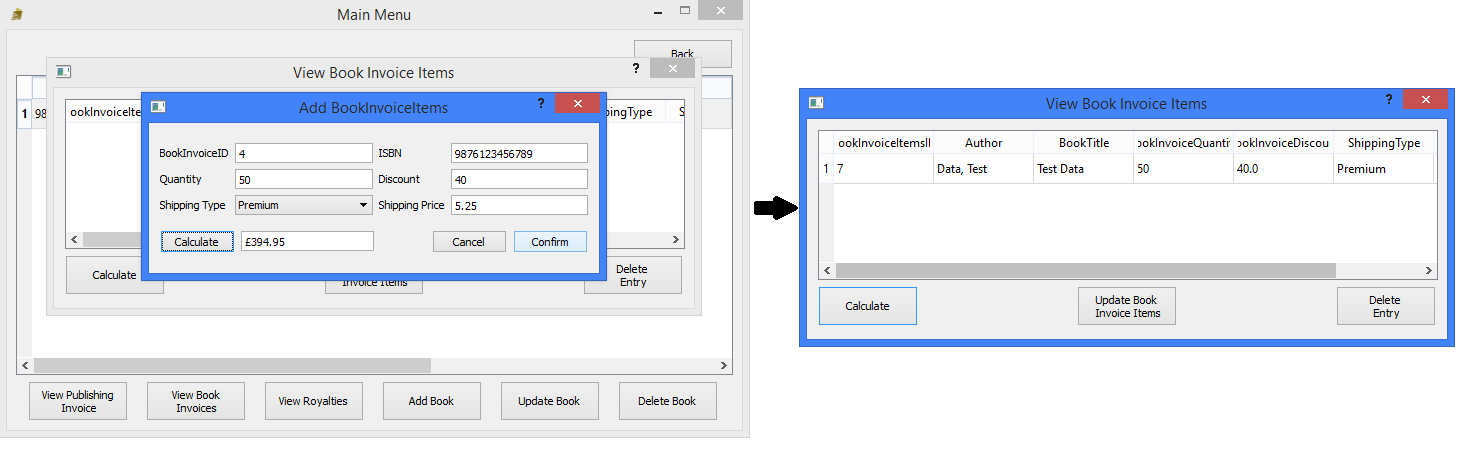
\includegraphics[width=\textwidth]{./Testing/Evidence/Series4/AddBookInvoiceItemsTest.png}
    \caption{Test 4.5 - Testing the process of adding Book Invoice Items}  \label{fig:AddBookInvoiceItemsTest}
\end{figure}

\begin{figure}[H]
    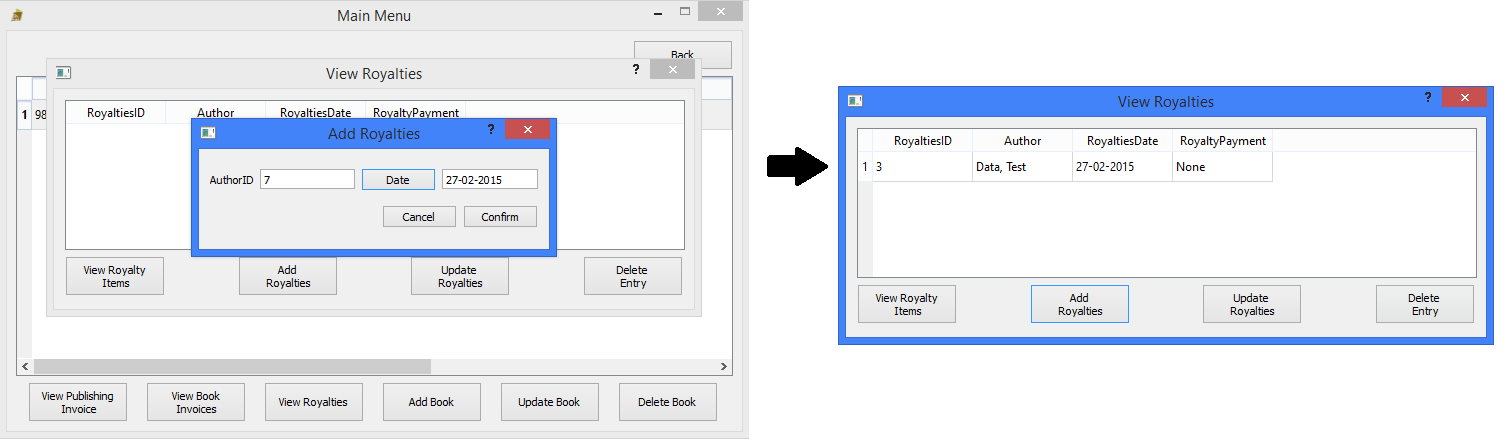
\includegraphics[width=\textwidth]{./Testing/Evidence/Series4/AddRoyaltiesTest.png}
    \caption{Test 4.6 - Testing the process of adding a Royalty Payment}  \label{fig:AddRoyaltiesTest}
\end{figure}

\begin{figure}[H]
    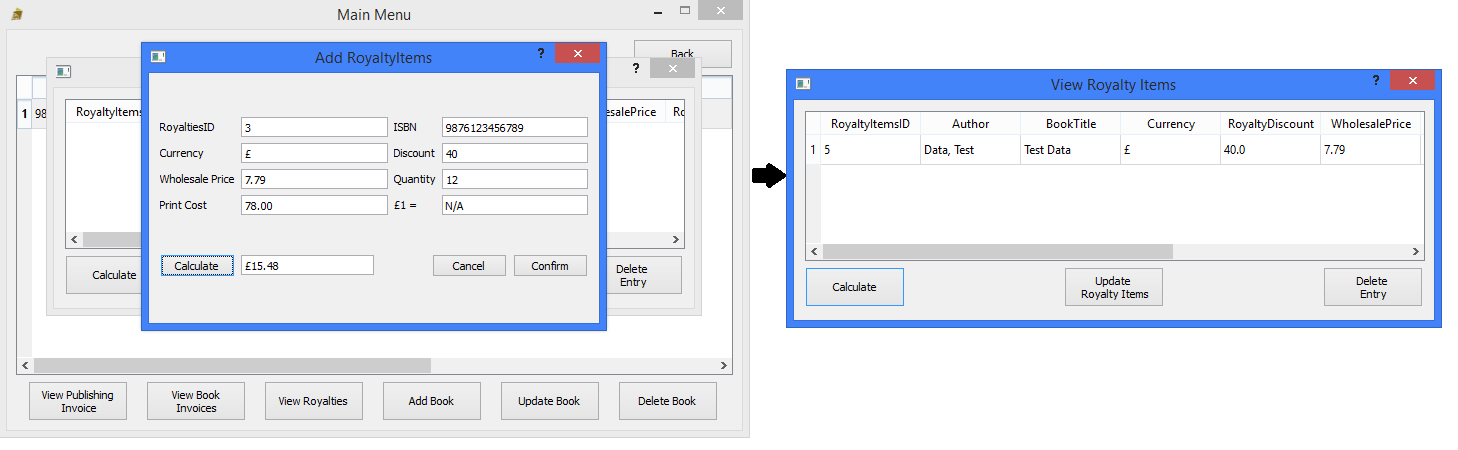
\includegraphics[width=\textwidth]{./Testing/Evidence/Series4/AddRoyaltyItemsTest.png}
    \caption{Test 4.7 - Testing the process of adding Royalty Items}  \label{fig:AddRoyaltyItemsTest}
\end{figure}

\begin{figure}[H]
    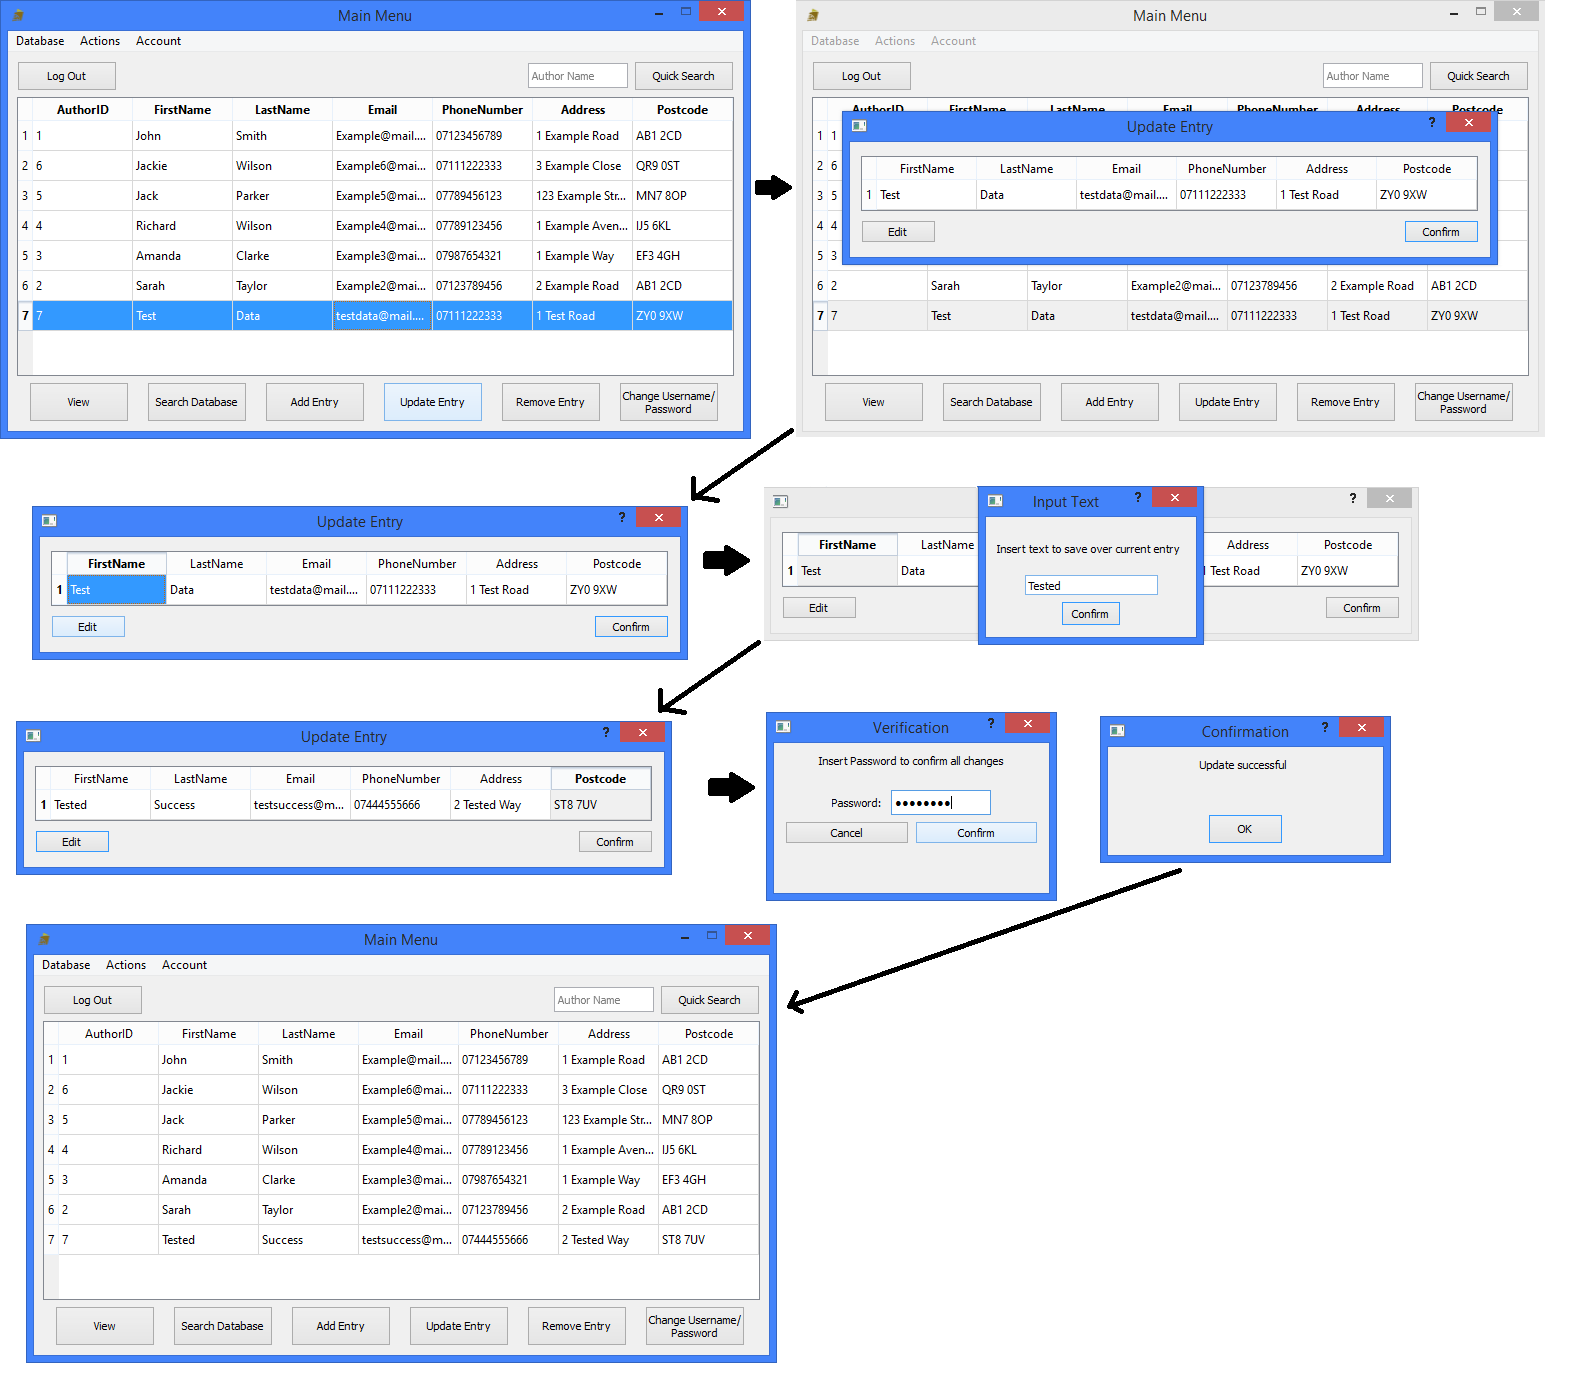
\includegraphics[width=\textwidth]{./Testing/Evidence/Series4/UpdateAuthorTest.png}
    \caption{Test 4.8 - Testing the process of Updating an Author}  \label{fig:UpdateAuthorTest}
\end{figure}

\begin{figure}[H]
    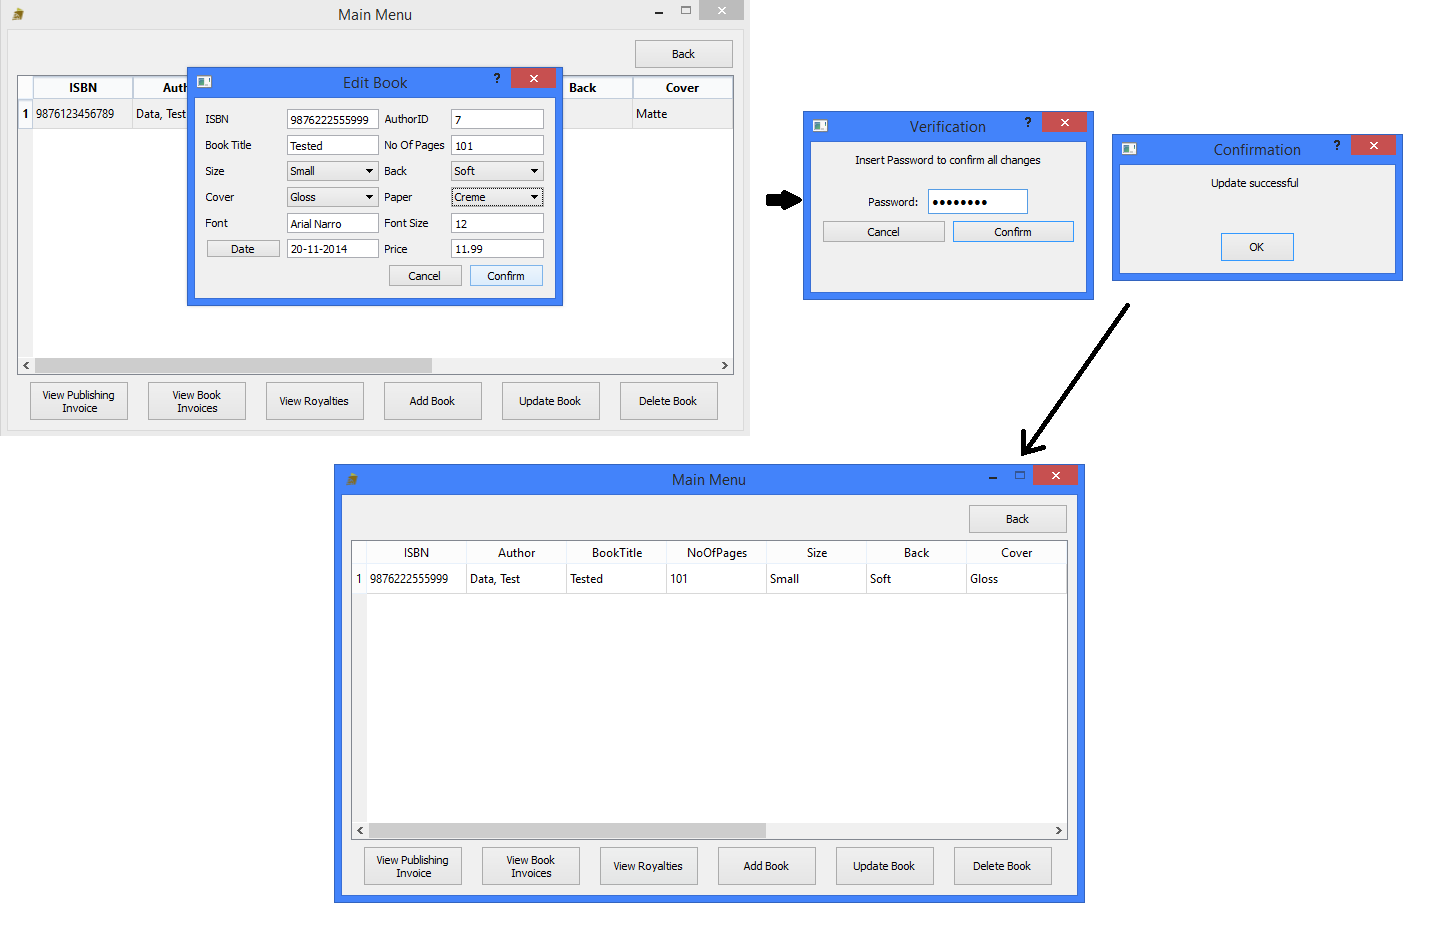
\includegraphics[width=\textwidth]{./Testing/Evidence/Series4/UpdateBookTest.png}
    \caption{Test 4.9 - Testing the process of Updating a Book}  \label{fig:UpdateBookTest}
\end{figure}

\begin{figure}[H]
    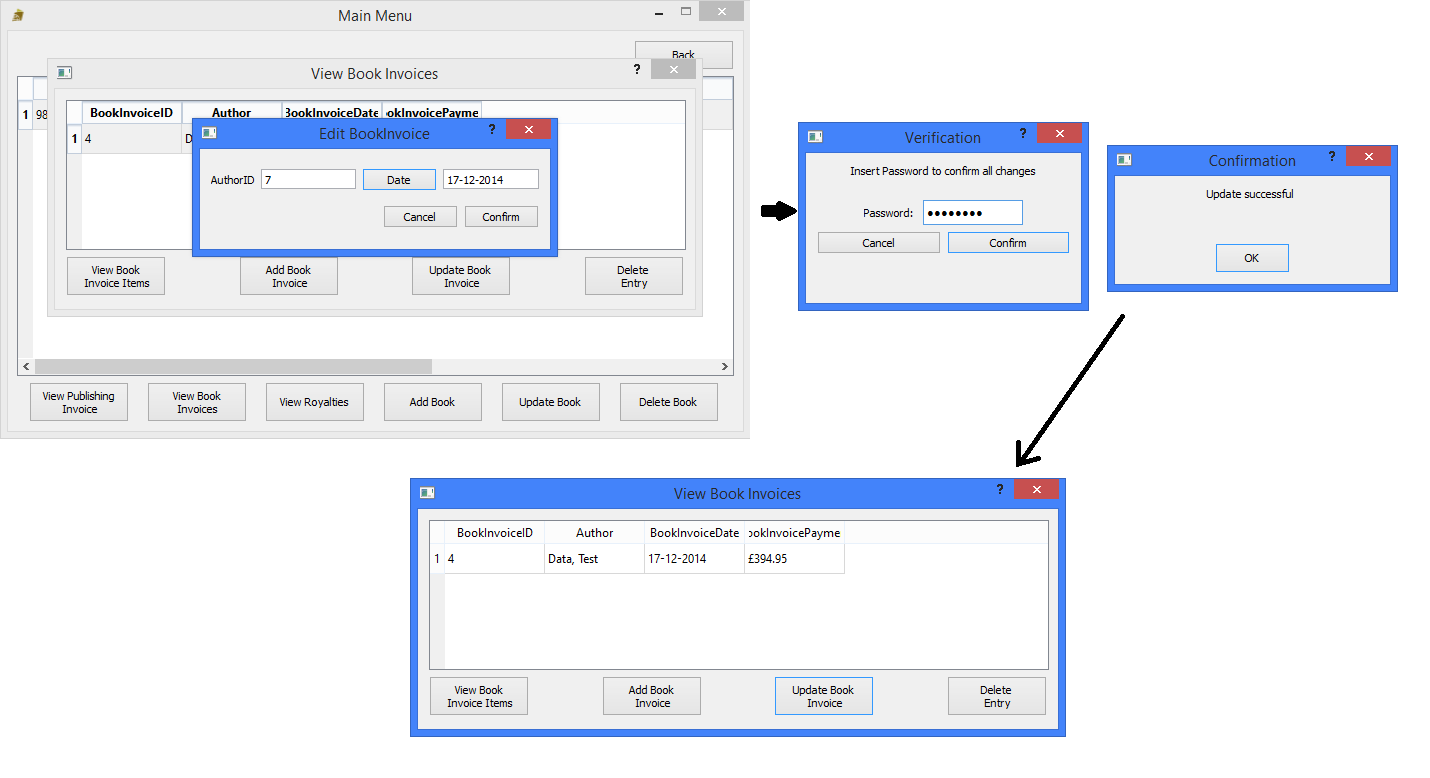
\includegraphics[width=\textwidth]{./Testing/Evidence/Series4/UpdateBookInvoiceTest.png}
    \caption{Test 4.10 - Testing the process of Updating a Book Invoice}  \label{fig:UpdateBookInvoiceTest}
\end{figure}

\begin{figure}[H]
    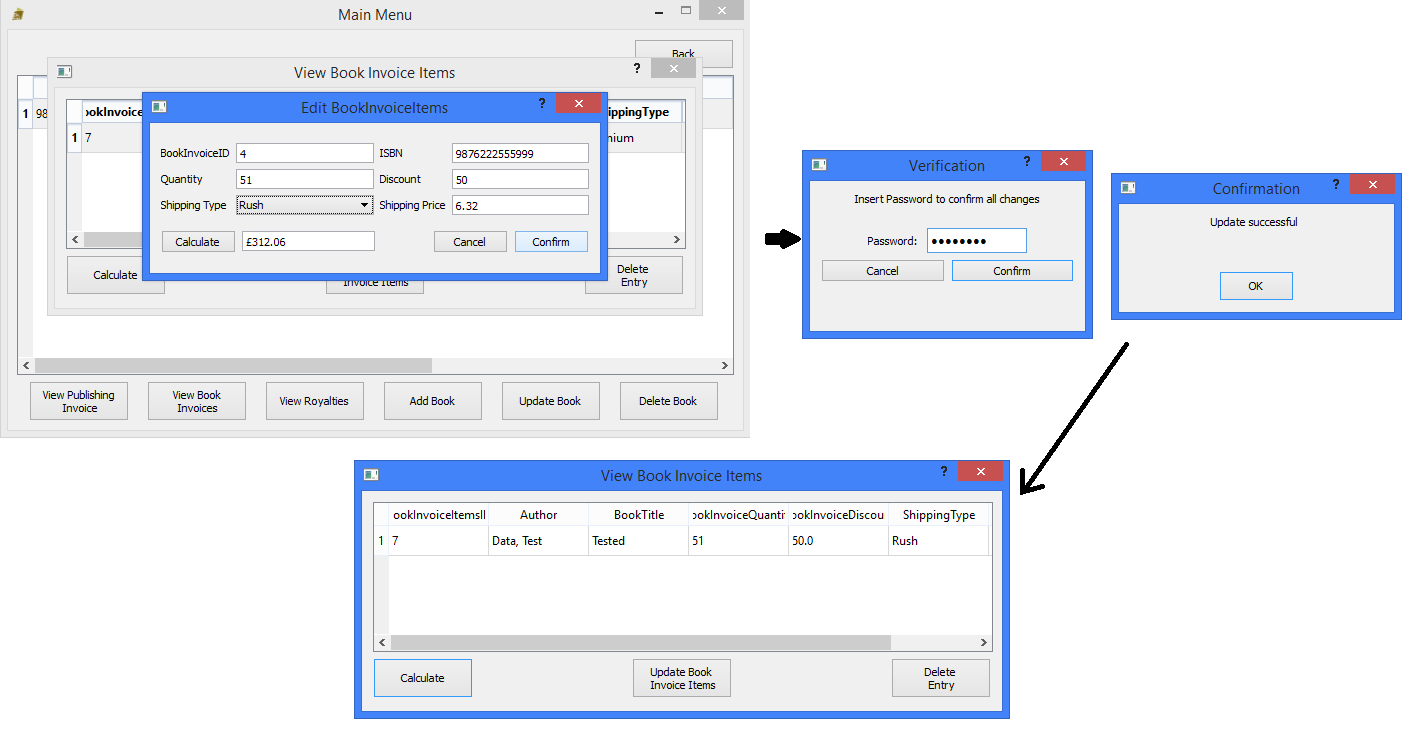
\includegraphics[width=\textwidth]{./Testing/Evidence/Series4/UpdateBookInvoiceItemsTest.png}
    \caption{Test 4.11 - Testing the process of Updating Book Invoice Items}  \label{fig:UpdateBookInvoiceItemsTest}
\end{figure}

\begin{figure}[H]
    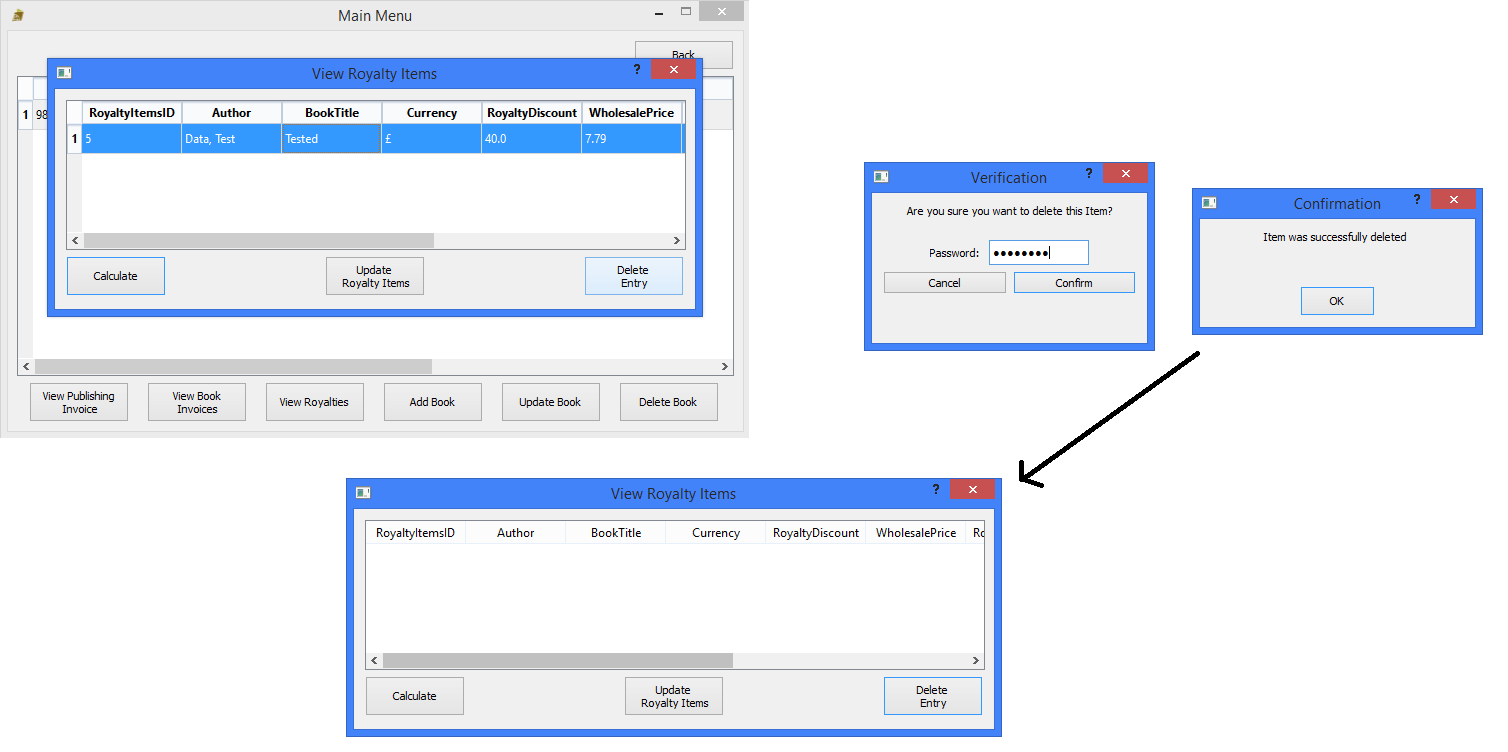
\includegraphics[width=\textwidth]{./Testing/Evidence/Series4/DeleteRoyaltyItemsDataTest.png}
    \caption{Test 4.12 - Testing the process of Deleting Royalty Items}  \label{fig:DeleteRoyaltyItemsDataTest}
\end{figure}

\begin{figure}[H]
    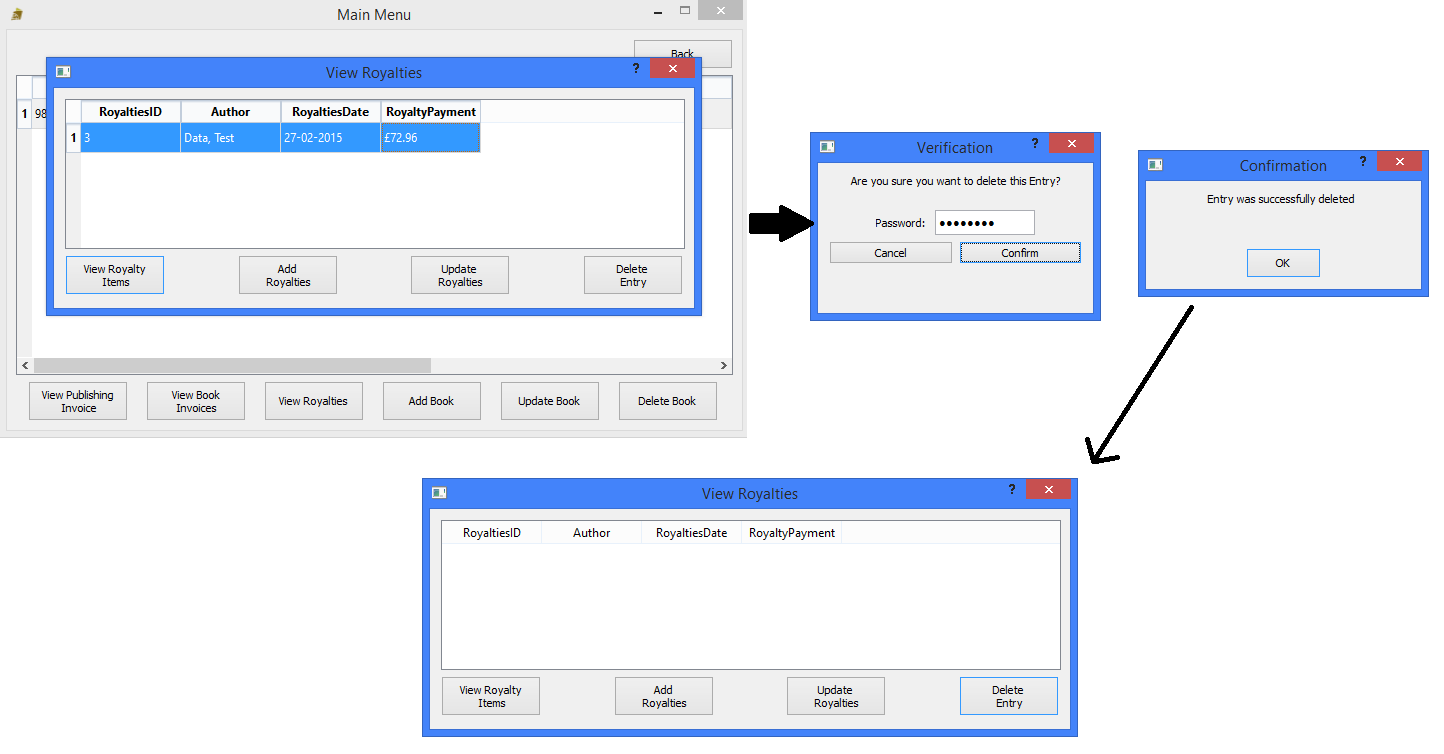
\includegraphics[width=\textwidth]{./Testing/Evidence/Series4/DeleteRoyaltiesDataTest.png}
    \caption{Test 4.13 - Testing the process of Deleting a Royalty Payment}  \label{fig:DeleteRoyaltiesDataTest}
\end{figure}

\begin{figure}[H]
    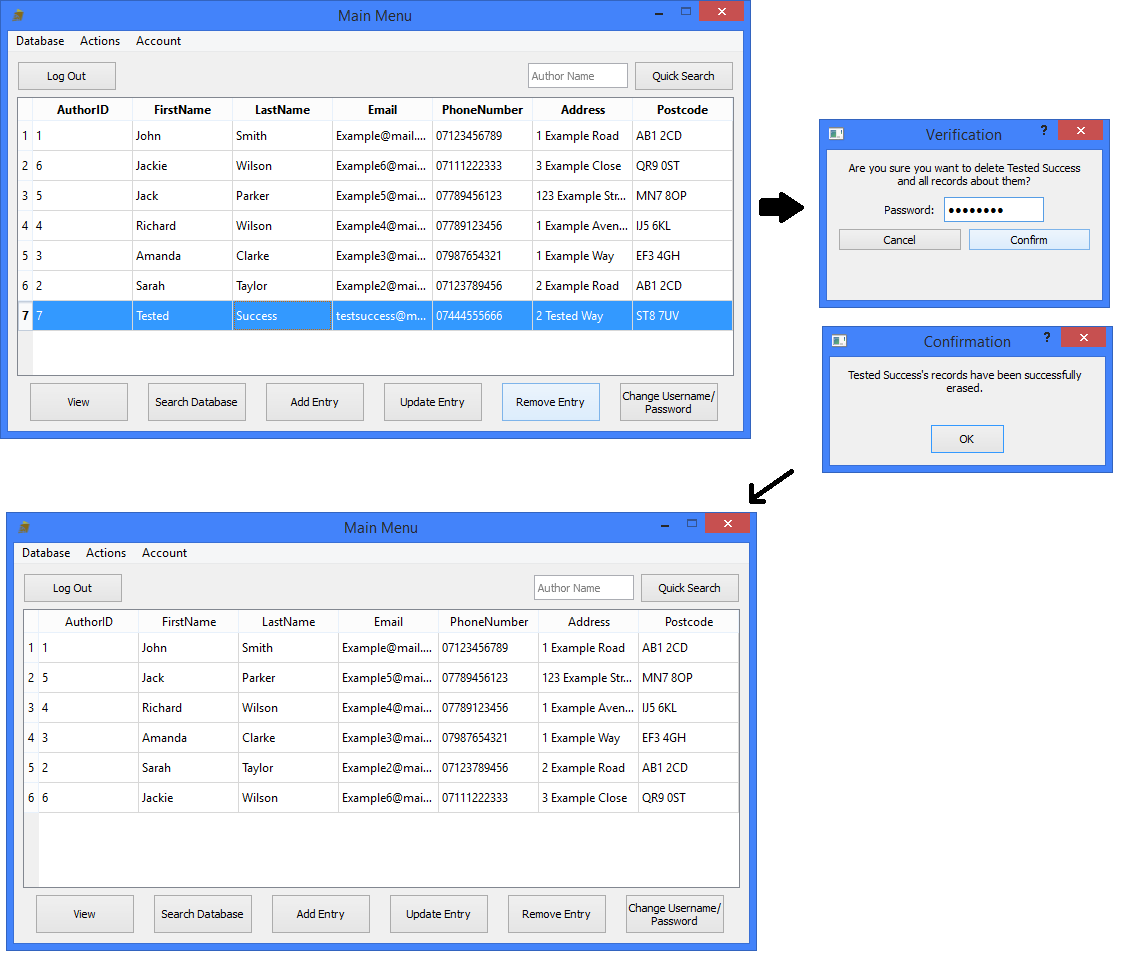
\includegraphics[width=\textwidth]{./Testing/Evidence/Series4/DeleteAuthorDataTest.png}
    \caption{Test 4.14 - Testing the process of Deleting an Author and all data linked with it}  \label{fig:DeleteAuthorDataTest}
\end{figure}

\end{landscape}

\section{Evaluation}

\subsection{Approach to Testing}

I have chosen to use a range of testing strategies. For instance, series 1 of of the tests is testing the flow of control, making sure that the user navigates to the correct areas of the interface. Series 2 of the tests ensures that the validation of user inputs is performed correctly, whilst series 3 certifies that the calculations and algorithms in the system function correctly. Series 4 makes sure that the added data is stored correctly, updated data is saved to the correct tables and fields, and the deletion of data is performed on the correct data. 

\subsection{Problems Encountered}

I encountered a few minor problems whilst testing my program.

\underline{Tests 2.9 and 2.10}, Figures \ref{fig:BookInvoiceDiscountValidation} and \ref{fig:RoyaltyDiscountValidation} on pages \pageref{fig:BookInvoiceDiscountValidation} and \pageref{fig:RoyaltyDiscountValidation} respectively

These tests encountered a minor problem, where if the user were to enter an invalid value for an entry, proceed to calculate using their inputs and confirm that they wish to add it to the database, the user would be correctly prompted with an error. However, upon dismissing the error, the window that they were using to add data to the database would close, forcing them to reopen the window and start entering data again. I have a vague idea of where the problem is,  but as it isn't a serious problem for the user, this will be considered as an area for future updates. 

This is the only problem my tests encountered, which also affected a few of the tests in series 3, causing the same issue.


\subsection{Strengths of Testing}

The strengths of my testing program consisted mainly of the consistency of the flow of data, and the flow of control. This proved that there wouldn't be any problem with the navigation of the user interface, and also no problems would be encountered when interacting with the data. Also, the testing program concluded that the user was limited to certain inputs for certain fields. For example, the user was required to enter a discount for the Book Invoice Items, and was limited to being able to enter numbers alone. This is seen in the evidence for test 2.9, Figure \ref{fig:BookInvoiceDiscountValidation} on page \pageref{fig:BookInvoiceDiscountValidation}. Also, dropdown lists were used to prevent the user from incorrectly spelling certain inputs. This can be seen in a number of my examples of evidence, such as Figure \ref{fig:AddBookTest} on page \pageref{fig:AddBookTest} for test 4.2 and Figure \ref{fig:UpdateBookInvoiceItemsTest} on page \pageref{UpdateBookInvoiceItems} for test 4.11. This showed that the testing program would not be limited to identifying specific errors as the user was prevented from entering incorrect data in some parts of the program.

\subsection{Weaknesses of Testing}

A weakness of my testing program was that it did not test every single component of the system. because most of the program used similar coding for its functionality. Therefore, after testing a few of the components, others were not tested because of the similar functionality. For example, a number of windows for adding, editing and deleting have a cancel button to close the window. I have only tested two of these, as I can gain the assumption that all the cancel buttons work to the required standard fromm testing to see whether these two work. This can be seen in tests 1.25 and 1.26, where I tested these cancel buttons. This means that I am unable to establish that the system is entirely robust.

\subsection{Reliability of Application}

All inputs, outputs and changes function as the should do, and as they were planned to. The system mostly prevents te user from entering inaccurate data, so that the inputs and outputs would not malfunction. Although, test 3.4 shows that a calculation would still be conducted if the user had entered a negative number, which is invalid. This happened because the calculation is conducted immediately after the user types. However, the program would not allow the user to confirm their entry with this invalid data, despite the calculations being conducted. This can be seen in the evidence for test 2.9, Figure \ref{fig:BookInvoiceDiscountValidation} on page \pageref{fig:BookInvoiceDiscountValidation} where a calculation is conducted, but the user is prompted against the invalid entry. Consequently, the system is generally reliable as it is moderately effective in preventing invalid entries.

\subsection{Robustness of Application}

The testing program used proves that the system is fairly robust. The program never encounters runtime errors or index errors, which were carefully prevented during the development of my system. Also, the system prevents invalid entries so that the program doesn't crash, as seen in the evidence for test 2.6, Figure \ref{fig:InvalidAddress} on page \pageref{fig:InvalidAddress},  and my test program did not cause my system to crash once.